\chapter{The Theory} \label{chap:chap-2}

% epigraph after chapter heading
% \epigraph{Some, I assume, are good people...}{-- Andrei Gritsan}

% %%%% MUST: if the chapter is a reprint or submitted paper, you must declare it
% %% you can use enumerate or itemize environment if you have more than one paper 
% %% \mybibexclude{} will exclude this citation from the final bibliography
% %% if this paper appears somewhere else then remove \mybibexclude{} command

% \begin{singlespace}         % you can also use `onehalfspace` to relax the spacing
%     This chapter is adapted from the following article with permission from <publisher>
    
%     \fullcite{einstein}. \mybibexclude{einstein}
% \end{singlespace} 


%%%% remove the following and add your chapter text here

\section{The Standard Model of Particle Physics}


\subsection{Elementary Particles}

Elementary particles are the most fundamental constituents of the universe, forming the basis of all known matter and mediating the fundamental forces that govern physical interactions. These particles, as described by the Standard Model (SM) of particle physics illustrated in Figure~\ref{fig:standardmodel}, are not composed of any smaller constituents that we know of and are broadly classified into fermions, which constitute matter, and bosons, which mediate interactions. 

Fermions are divided into two distinct families: quarks and leptons. A fundamental property of quarks is color charge, which confines them within composite particles called hadrons, preventing their isolation in nature. They come in six flavors---up, down, charm, strange, top, and bottom---each possessing unique masses and charge properties. Quarks are susceptible to all fundamental forces, but interact predominantly via the strong force, which grows stronger as quarks attempt to separate, ensuring that they exist as elementary components of color-neutral bound states such as baryons (e.g., protons and neutrons) and mesons (e.g., pions). 

Leptons, unlike quarks, are elementary particles that do not experience the strong force. The three charged leptons—electron, muon, and tau—interact via the electromagnetic and weak forces, while their corresponding neutrinos (electron neutrino, muon neutrino, and tau neutrino) interact only through the weak force. Neutrinos are particularly intriguing due to their extremely small masses and their ability to oscillate between different flavors.

% \begin{figure}
% \centering
% \includesvg[scale=0.4]{figures/Standard_Model_of_Elementary_Particles.svg}
% \caption{Particle content of the Standard Model.}
% \label{fig:standardmodel}
% \end{figure}

\begin{figure}
\centering
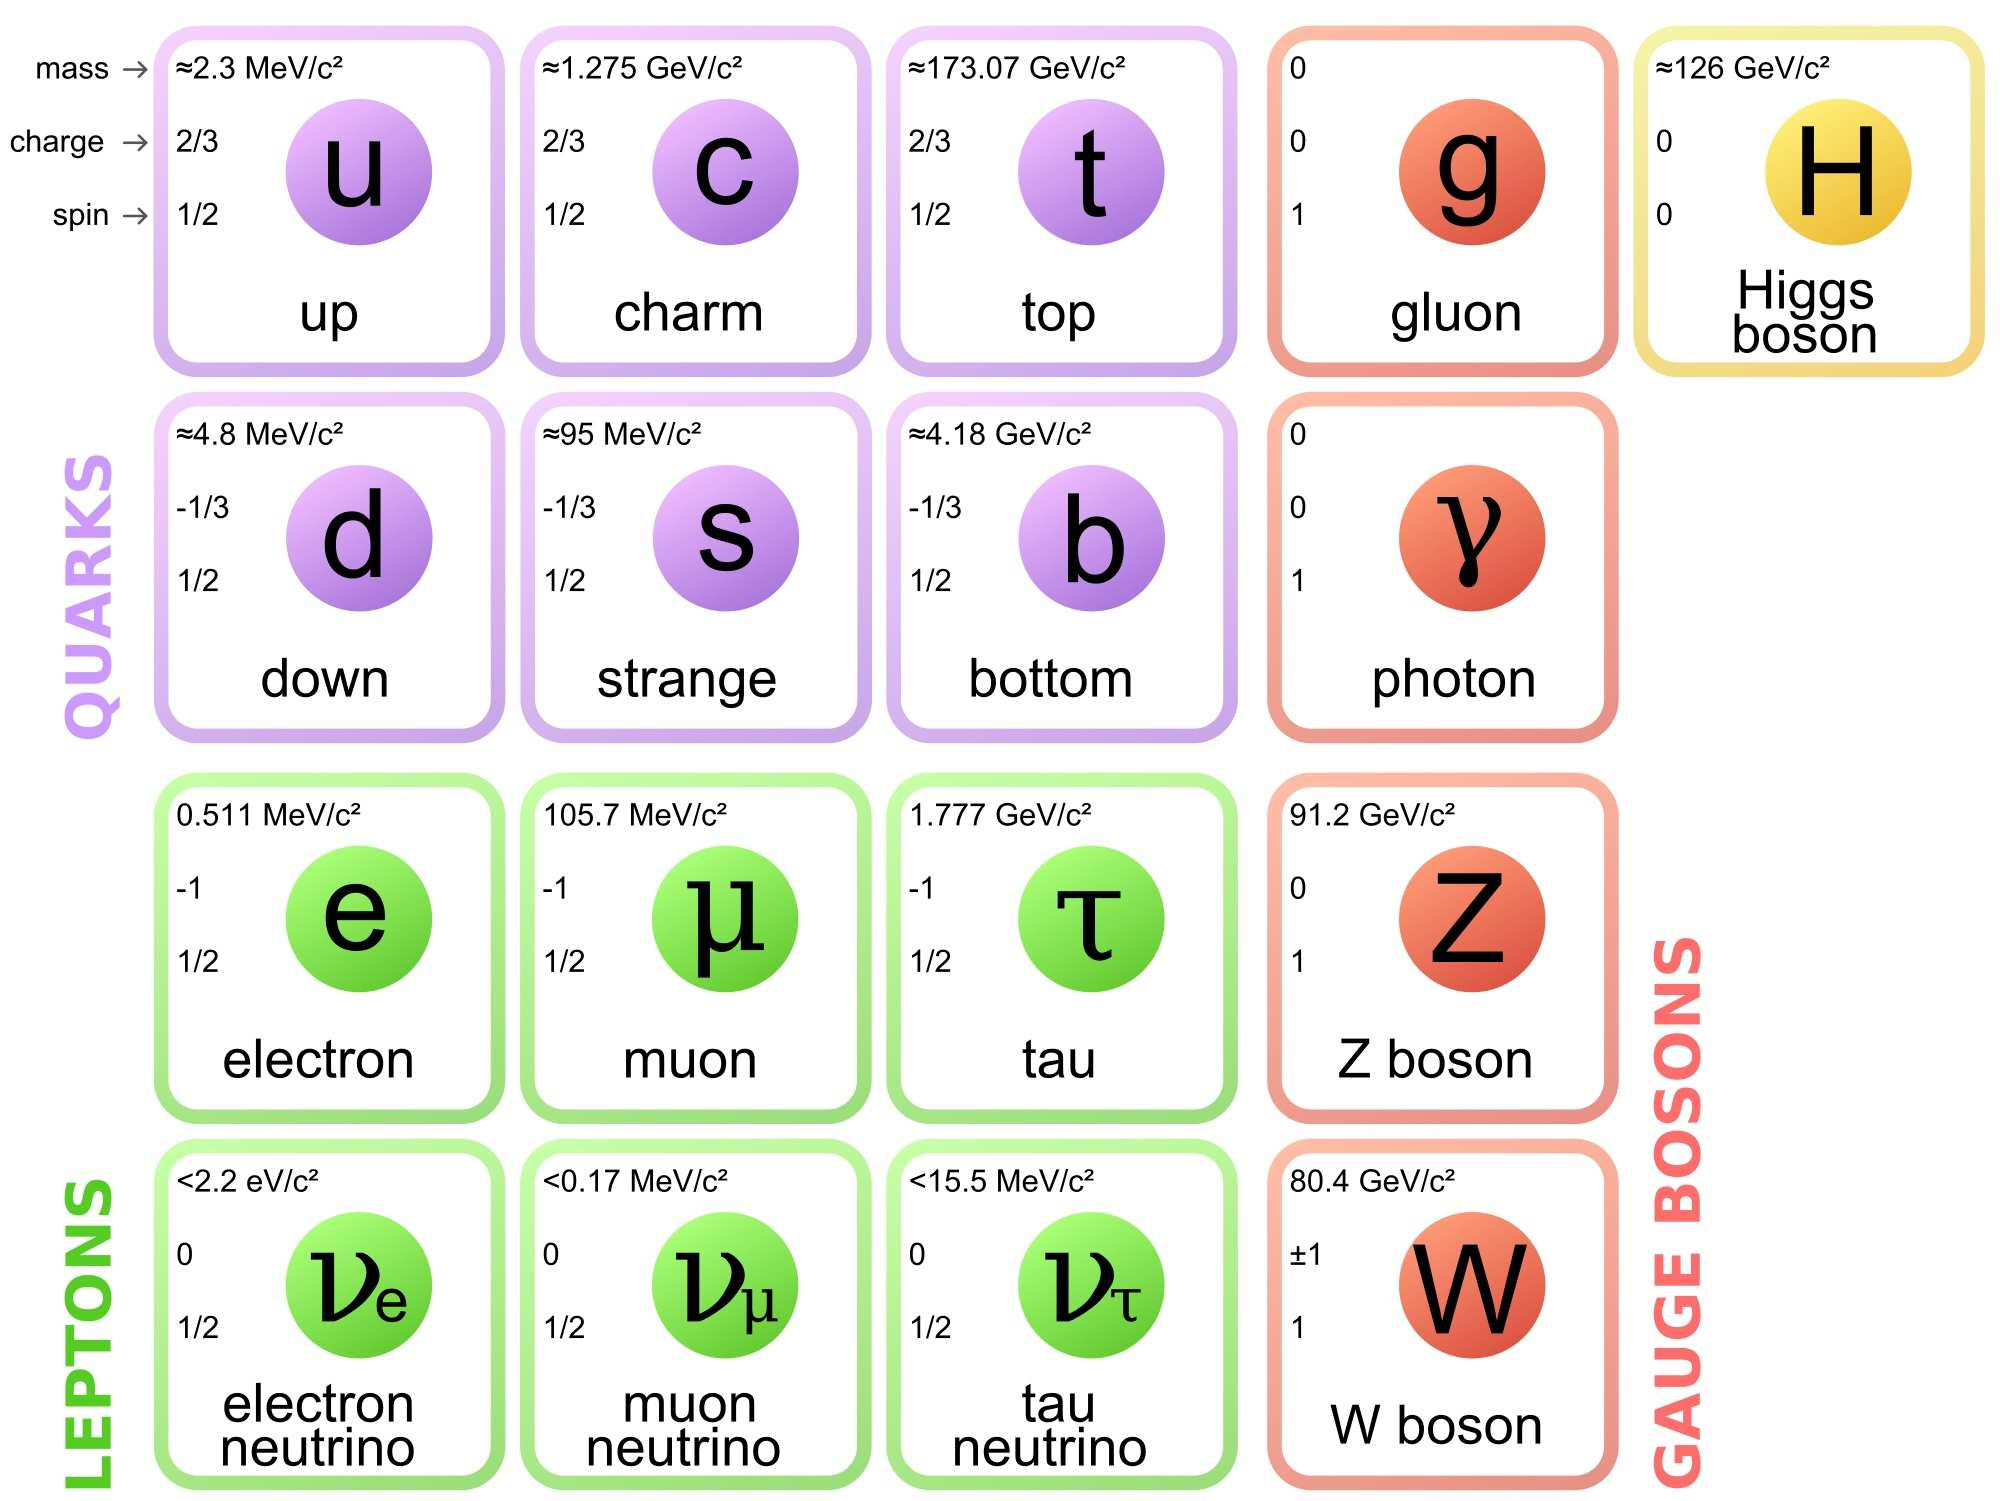
\includegraphics[width=0.9\textwidth,clip] {figures/2000px-Standard_Model_of_Elementary_Particles.png}
\caption{Particle content of the Standard Model.}
\label{fig:standardmodel}
\end{figure}

\subsection{Forces and Symmetries}

% Fundamental interactions in quantum field theory arise from the exchange of gauge bosons, which mediate the four fundamental forces at work in the universe: the strong force, the weak force, the electromagnetic force, and the gravitational force. They work over different ranges and have different strengths: gravity is the weakest but it has an infinite range; the electromagnetic force also has infinite range but it is many times stronger than gravity; the weak and strong forces are effective only over a very short range and dominate at the level of subatomic particles. Despite its name, the weak force is actually much stronger than gravity, though it is indeed the weakest of the other three. The strong force, as the name suggests, is the strongest of all four fundamental interactions.

Fundamental interactions in quantum field theory arise from the exchange of gauge bosons, which mediate three of the fundamental forces at work in the universe: the strong force, the weak force, and the electromagnetic force. They work over different ranges and have different strengths: the electromagnetic force has infinite range and can predominantly drive interactions at intermediate scales; the weak and strong forces are effective only over a very short range and dominate at the level of subatomic particles. The weak force is so named because it is the weakest of the three forces at the scale of partons like quarks. The strong force, as the name suggests, is the strongest of all fundamental interactions between elementary particles at similar scale. 

The strong nuclear force is mediated by gluons, which carry the force that binds quarks together to form protons, neutrons, and other hadrons. Unlike other force carriers, gluons themselves possess color charge, allowing them to interact with one another. At nuclear scales (approximately 1–3 femtometers), a residual effect of this fundamental force termed the ``nuclear force,'' carried by mesons such as pions, binds protons and neutrons together to form atomic nuclei. 

The electromagnetic force, responsible for interactions between electrically charged particles, is mediated by photons. This force contributes to macroscopic interactions at various scales, from atomic bonding to everyday life (though significantly larger scales are dominated by gravity), and has an infinite range, diminishing in strength with the inverse square of the distance. The electromagnetic force is vastly stronger than gravity but is often neutralized at larger scales due to the balance of positive and negative charges in matter.

The weak interaction, mediated by the W and Z bosons, governs processes such as beta decay, or neutrino interactions. %, and other flavor-changing reactions. 
The W bosons facilitate charged-current interactions, enabling quarks to change flavor (e.g., converting a neutron into a proton in beta decay) or transforming a lepton into its corresponding neutrino. The Z boson mediates neutral-current interactions, which do not change particle identities but influence their scattering behavior. Unlike the strong and electromagnetic forces, the weak force has a highly limited range ($10^{-18}$ meters), due to the large masses of the W and Z bosons, which restrict their influence.  

% Quarks are held together by gluons, which provide protons and neutrons mass. Quarks can shoot off gluons, since gluons are the mediators of the strong force. The strong interaction is observable at two ranges and mediated by two force carriers. On a larger scale (about 1 to 3 fm), it is the force (carried by mesons like pion which can change neutron to proton and vice versa) that binds protons and neutrons (nucleons) together to form the nucleus of an atom. On the smaller scale (less than about 0.8 fm, the radius of a nucleon), it is the force (carried by gluons) that holds quarks together to form protons, neutrons, and other hadron particles.

% Electrically charged particles can emit photons, which are the mediators of the electromagnetic force.

% Quarks, leptons, and neutrinos can emit Z and W bosons, as mediators of the weak force. W bosons deal with charged-current interactions and are responsible for beta decay (by changing the flavor of a quark in a proton, for example, turning it into a neutron, and then decaying to a positron and electron neutrino) or for turning a lepton into its neutrino (weak isospin differs by 1). Z bosons deal with neutral-current interactions and is responsible for deflection/elastic collisions.

%====================================================================================================

% The weak force is essentially as strong as the electromagnetic force, but it appears weak because its influence is limited by the large mass of the Z and W bosons. Their mass limits the range of the weak force to about 10-18 metres, and it vanishes altogether beyond the radius of a single proton.

% Three of the fundamental forces result from the exchange of force-carrier particles, which belong to a broader group called “bosons”. Particles of matter transfer discrete amounts of energy by exchanging bosons with each other. The strong force is carried by the “gluon”, the electromagnetic force is carried by the “photon”, and the “W and Z bosons” are responsible for the weak force.

% But why are the nuclear forces not long-range forces? 
% Goldstone proved that you can break symmetries by putting a field in empty space. But then even if you give masses to the gauge bosons, you get massless Goldstone bosons. 
% Goldstone's theorem seemed to imply that if you had a symmetry in some form, you would always end up with a massless particle. 
% Thus it was thought that the nuclear forces could not be Yang-Mills theories (based on gauge symmetries) because that would necessarily lead to massless particles, which were definitely not observed in laboratory settings. 

% However, this logic was flawed. In the case of the strong nuclear force, gluons interact with each other. 
% Photons of electromagnetism interact with electrically charged particles, but the photons themselves are not electrically charged.
% However, gluons interact with colored particles, such as quarks, while also being colored themselves. This means that gluons inside nuclei are interacting with each other and this leads to a phenomenon called ``confinement.'' 
% From outside the proton, there’s almost no evidence of the strong nuclear force, but inside a proton it is very strong.

% A different mechanism makes the weak nuclear force short range. 
% The Higgs field fills space and absorbs the weak nuclear force, giving mass to the W and Z bosons.

% The weak nuclear force, while comparable in intrinsic coupling strength to the electromagnetic interaction, appears much weaker at macroscopic scales due to the large mass of its mediating gauge bosons, the W and Z. Unlike the photon, which is massless and therefore allows electromagnetic forces to propagate over infinite distances, the W and Z bosons have masses on the order of 80 and 90 GeV, respectively. This mass constrains the weak interaction to a characteristic range of approximately $10^{-18}$ meters, comparable to the spatial extent of a nucleon. At distances beyond this range, the weak force is exponentially suppressed, effectively vanishing at scales larger than the atomic nucleus.

% Fundamental interactions in quantum field theory arise from the exchange of gauge bosons, which mediate forces between elementary particles. The electromagnetic force is governed by the exchange of photons, which couple to electrically charged particles, while the strong nuclear force is mediated by gluons, which interact with quarks and with each other due to their color charge. The weak interaction, responsible for flavor-changing processes such as beta decay, is carried by the massive W and Z bosons. The key difference between these interactions lies in the properties of their force carriers: the photon and gluons are massless, allowing their respective forces to operate over long or effectively infinite distances, whereas the W and Z bosons acquire mass through the Higgs mechanism, thereby restricting the weak force to subnuclear scales.

A fundamental question in early quantum field theory was why the strong and weak interactions are not long-range, and why there exists only a residual nuclear force outside the proton. Goldstone’s theorem, a critical result in quantum field theory, originally suggested that any spontaneously broken continuous symmetry would necessarily yield massless scalar bosons~\cite{Griffiths:1987tj}. This posed a major theoretical challenge, as no such massless particles were observed in experiments involving the weak force. It was thus believed that Yang-Mills gauge theories, which rely on local symmetries, could not correctly describe the weak interaction, since they would seemingly predict unobserved massless bosons.

However, this reasoning was incomplete. In the case of the strong interaction, the resolution lies in the non-abelian nature of quantum chromodynamics (QCD). Unlike electromagnetism, where photons interact with charged particles but remain neutral themselves, gluons possess color charge and therefore interact not only with quarks but also with each other. This self-interaction of gluons inside nuclei gives rise to ``confinement:'' quarks and gluons are permanently bound within hadrons such as protons and neutrons, and the strong force does not manifest significantly beyond nucleonic scales. While the strong force is immensely powerful at short distances, its effects are effectively screened at larger distances and from outside the proton, there’s almost no evidence of the strong force.

However, a completely different mechanism is responsible for the short range of the weak force. It turns out that the Higgs field, which permeates all of space, undergoes spontaneous symmetry breaking, providing a mass mechanism for the weak gauge bosons. In the SM, the electroweak symmetry group $SU(2)_L \times U(1)_Y$ is spontaneously broken to the electromagnetic subgroup $U(1)_{\text{EM}}$ by the Higgs vacuum expectation value, or VEV. This breaking mechanism gives mass to the W and Z bosons while leaving the photon massless, thereby allowing electromagnetism to remain long-range while restricting the weak force to subatomic scales. Despite the weak interaction's intrinsic coupling strength, the large masses of its mediators ensure that weak processes occur only over extremely short distances, making the weak force appear weak at macroscopic scales.

%====================================================================================================

% Philip Anderson in 1963 (Plasmons, Gauge Invariance, and Mass) proposed a field filling space that could give weak interaction bosons a mass and explain why they were not long range.
% Then in 1964 (Broken Symmetry and the Mass of Gauge Vector Mesons), physicists Francois Englert and Robert Brout proposed the idea that is now called the Higgs mechanism.

% Also 1964, ``Broken Symmetries and the Masses of Gauge Bosons'' by Peter Higgs, and ``Global Conservation Laws and Massless Particles'' by Gerald Guralnik, Carl Hagen, and Tom Kibble.

% In 1967 (A Model of Leptons), Steven Weinberg wrote a paper that took the idea of the Higgs mechanism and showed how it explained the weak interactions. Weinberg took Glashow’s model--with enough symmetry to give you the W bosons, the Z boson, and the photon--and used the Higgs field to break those symmetries.

% Similar proposal of Glashow’s model by another physicist named Abdus Salam. Nobel for the electroweak theory was shared by Glashow, Weinberg, and Salam.

% 1971 ``Renormalization of massless Yang-Mills fields'' and ``Renormalizable Lagrangians for massive Yang-Mills fields'' by Gerard 't Hooft.

% The ``ABEGHHK’tH'' boson in stead of the ``Higgs'' boson. 

% The Higgs field permeates all of space and plays a crucial role in electroweak symmetry breaking, providing mass to the weak interaction bosons while leaving the photon massless. This mechanism is fundamental to the Standard Model, explaining why the weak nuclear force operates over a short range while the electromagnetic force remains long-ranged. The theoretical formulation of this idea emerged gradually over several decades, incorporating insights from multiple physicists and culminating in the eventual discovery of the Higgs boson in 2012.

\section{The Higgs Mechanism} \label{sec:higgs}

The origins of the Higgs mechanism can actually be traced to condensed matter physics, where Philip Anderson, in his 1963 paper on gauge invariance in superconductors, suggested that a field permeating space could confer mass to otherwise massless gauge bosons. This idea laid the groundwork for the development of a relativistic field-theoretic framework that could explain the mass of weak interaction bosons.

In 1964, several independent groups formalized this concept within the context of particle physics. François Englert and Robert Brout first published a paper describing spontaneous symmetry breaking in gauge theories, demonstrating how vector bosons could acquire mass without violating gauge invariance. Shortly thereafter, Peter Higgs elaborated on this mechanism and explicitly predicted the existence of a new scalar boson, now known as the Higgs boson. Around the same time, Gerald Guralnik, Carl Hagen, and Tom Kibble presented an alternative but equivalent formulation of the same underlying physics. This collective work established what is now recognized as the Higgs mechanism.

In 1967, Steven Weinberg incorporated the Higgs mechanism into electroweak theory, building upon Sheldon Glashow’s earlier work. Glashow had introduced a unified framework for the weak and electromagnetic interactions, postulating the existence of the W and Z bosons along with the photon. However, his model required a mechanism to break symmetry while preserving gauge invariance. Weinberg demonstrated that the Higgs field could accomplish this, allowing for the spontaneous breaking of electroweak symmetry and thereby endowing the W and Z bosons with mass while keeping the photon massless. Around the same time, Abdus Salam independently developed a similar theory. The electroweak theory, formulated by Glashow, Weinberg, and Salam, was instrumental in shaping the SM and earned the three physicists the 1979 Nobel Prize in Physics.

A major hurdle for early versions of the electroweak theory was the question of renormalizability—whether the theory could yield finite, predictive results at all energy scales. In 1971, Gerard ’t Hooft, under the supervision of Martinus Veltman, demonstrated that gauge theories with spontaneously broken symmetry, including the electroweak theory, were renormalizable. This work provided the final theoretical validation of the SM framework and solidified the Higgs mechanism as a cornerstone of modern particle physics.

Although widely referred to as the Higgs boson, some physicists have suggested that its name should reflect the collective contributions of multiple researchers. The term ``ABEGHHK’tH boson'' has been proposed, incorporating the initials of Anderson, Brout, Englert, Guralnik, Hagen, Higgs, Kibble, and ’t Hooft. However, historical convention has cemented the use of ``Higgs boson'' in both scientific and popular discourse.

%====================================================================================================

% The Higgs boson is not a gauge boson. In particular, the spin of the Higgs is zero, making it a scalar. This scalar boson is associated with the Higgs field, a scalar field that permeates all of space. Mathematically, the Higgs field $\phi$ is a complex scalar field with four degrees of freedom:
% \[
% \phi = \begin{pmatrix} \phi^+ \\ \phi^0 \end{pmatrix}.
% \]

% The field undergoes a spontaneous symmetry breaking due to the potential:
% \[
% V(\phi) = \mu^2|\phi|^2 + \lambda|\phi|^4,
% \]
% where $\mu^2 < 0$ and $\lambda > 0$. The negative mass term ($\mu^2 < 0$) causes the field to acquire a nonzero vacuum expectation value (VEV):
% \[
% \langle \phi \rangle = \begin{pmatrix} 0 \\ v/\sqrt{2} \end{pmatrix},
% \]
% where $v \approx 246\,\mathrm{GeV}$ is the VEV.




% The Higgs mechanism is the process by which gauge bosons in a spontaneously broken gauge theory acquire mass while maintaining gauge invariance. This mechanism is fundamental to the Standard Model (SM), where it explains the masses of the W and Z bosons and plays a crucial role in electroweak symmetry breaking (EWSB). Below, we outline the key mathematical aspects of the Higgs mechanism, including the Higgs scalar field, its potential, the vacuum expectation value (VEV), and how mass terms emerge for both vector bosons and fermions.

%====================================================================================================



In today's SM, the Higgs field is introduced as a complex scalar doublet under the electroweak gauge group \( SU(2)_L \times U(1)_Y \):

\begin{equation}
\label{eq:higgscalar}
    \Phi = \begin{pmatrix} \phi^+ \\ \phi^0 \end{pmatrix},
\end{equation}

where \( \phi^+ \) and \( \phi^0 \) are complex scalar fields. This field transforms under \( SU(2)_L \times U(1)_Y \) as \(\Phi \to e^{i\alpha^a \tau^a} e^{i\beta Y} \Phi,\) where \( \tau^a \) are the generators of \( SU(2) \), and \( Y \) is the hypercharge.

The dynamics of the Higgs field are governed by the Higgs potential:

\begin{equation}
\label{eq:higgpot}
V(\Phi) = \mu^2 \Phi^\dagger \Phi + \lambda (\Phi^\dagger \Phi)^2.
\end{equation}

The form of this potential depends on the sign of the real-valued parameter \( \mu^2 \). If \( \mu^2 > 0 \), the minimum of \( V(\Phi) \) occurs at \( \Phi = 0 \), preserving the full electroweak symmetry. If \( \mu^2 < 0 \), the potential acquires a ``Mexican hat'' shape, leading to spontaneous symmetry breaking (SSB) as illustrated in Figure~\ref{fig:mexicanhat}.

\begin{figure}[!hbt]
  \centering
  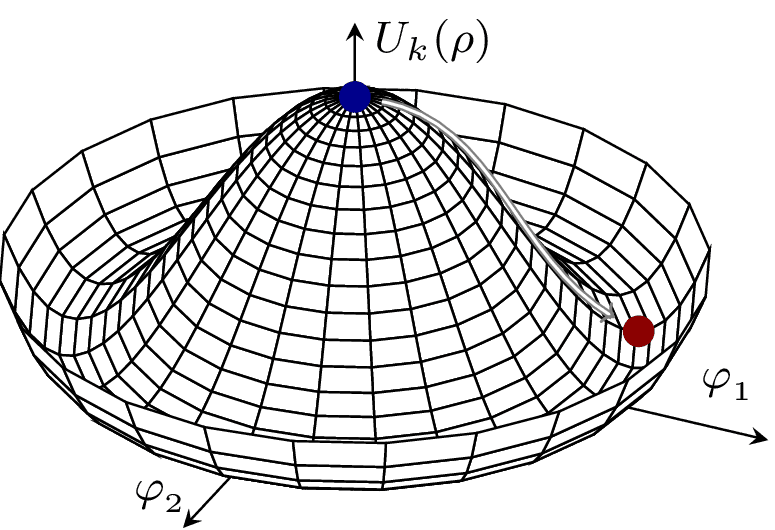
\includegraphics[width=0.75\textwidth,clip] {figures/mexican-hat.png}
    % \begin{tikzpicture}[font=\footnotesize]
    %   \begin{axis}[
    %       axis lines=center,
    %       axis equal,
    %       domain=0:360,
    %       y domain=0:1.25,
    %       y axis line style=stealth-,
    %       y label style={at={(0.35,0.18)}},
    %       xmax=1.6,zmax=1.3,
    %       xlabel = $\varphi_{_1}$,
    %       ylabel=$\varphi_{_2}$,
    %       zlabel=$U_k(\rho)$,
    %       ticks=none
    %     ]
    %     \addplot3 [surf,shader=flat,draw=black,fill=white,z buffer=sort] ({sin(x)*y}, {cos(x)*y}, {(y^2-1)^2});
    %     \coordinate (center) at (axis cs:0,0,1);
    %     \coordinate (minimum) at (axis cs:{cos(30)},{sin(30)},0);
    %   \end{axis}
    
    %   \fill[DarkBlue] (center) circle (0.1);
    %   \fill[DarkRed] (minimum) circle (0.1);
    %   \draw (center) edge[shorten <=5,shorten >=5,out=-10,in=150,double,draw=gray,double distance=0.5,-{>[length=2,line width=0.5]}] (minimum);
    % \end{tikzpicture}
  \caption{Visualization of the characteristic ``Mexican hat'' shaped Higgs potential, as parameterized by the two fields in the Higgs doublet.}
  % ~\cite{Thethril79:online}
  \label{fig:mexicanhat}
\end{figure}

For \( \mu^2 < 0 \), the Higgs field acquires a vacuum expectation value (VEV), breaking the electroweak symmetry:

\begin{equation}
\label{eq:higgssymmetry}
\langle \Phi \rangle = \frac{1}{\sqrt{2}} \begin{pmatrix} 0 \\ v \end{pmatrix}.
\end{equation}

Here, \( v \) is determined by minimizing the potential\footnote{Experimentally, the VEV is found to be approximately \( v \approx 246 \) GeV.}:

\begin{equation}
\label{eq:higgspotmin}
v = \sqrt{\frac{-\mu^2}{\lambda}}.
\end{equation}

The Higgs field interacts with the electroweak gauge bosons via the covariant derivative:

\begin{equation}
\label{eq:higgscovder}
D_\mu \Phi = \left( \partial_\mu - i g W^a_\mu \tau^a - i g' B_\mu Y \right) \Phi.
\end{equation}

Expanding around the VEV and extracting the quadratic terms in the Lagrangian, the mass terms for the gauge bosons emerge. The kinetic term for the Higgs field, 

\begin{equation}
\label{eq:higgskinetic}
(D_\mu \Phi)^\dagger (D^\mu \Phi),
\end{equation}

yields mass terms for the weak bosons:

\begin{equation}
\label{eq:higgsweakmass}
M_W = \frac{1}{2} g v, \quad M_Z = \frac{1}{2} \sqrt{g^2 + g'^2} v.
\end{equation}

The photon remains massless, as expected, since the Higgs mechanism only breaks \( SU(2)_L \times U(1)_Y \) down to \( U(1)_{\text{EM}} \).

Fermion masses arise through interactions of the Higgs field with the fermion fields. The strengths of these interactions are dictated by so-called Yukawa couplings, which take the form:

\begin{equation}
\label{eq:higgsyukawa}
\mathcal{L}_Y = - y_f \bar{\psi}_L \Phi \psi_R + \text{h.c.}
\end{equation}

After the Higgs field acquires a VEV, this interaction produces mass terms proportional to each fermion's Yukawa coupling strength \( y_f \):

\begin{equation}
\label{eq:higgsfermmass}
M_f = \frac{y_f v}{\sqrt{2}}.
\end{equation}

Thus, the Higgs mechanism provides a consistent and gauge-invariant way for the weak bosons and fermions to acquire mass while preserving renormalizability. The Higgs scalar field, through its spontaneous symmetry breaking, generates mass terms for the W and Z bosons, while fermions gain mass through Yukawa interactions. 

% The discovery of the Higgs boson at the LHC confirmed the validity of this mechanism and solidified the Standard Model's foundation, though open questions remain regarding the nature of electroweak symmetry breaking and possible physics beyond the Standard Model.

%====================================================================================================



% Through the Higgs mechanism, the interaction of particles with the Higgs field gives rise to their masses. Gauge bosons, such as the W and Z bosons, acquire masses proportional to $v$, while the photon remains massless. Fermions gain mass via Yukawa interactions:
% \[
% \mathcal{L}_\text{Yukawa} = -y \bar{\psi} \phi \psi ,
% \]
% where $y_f$ is the Yukawa coupling for a fermion $f$. The masses of fermions are proportional to $y_f v$.



%====================================================================================================
% HIGGS COCKTAIL PARTY ANALOGY
%====================================================================================================


% \begin{figure}[!hbt]
% \centering
% 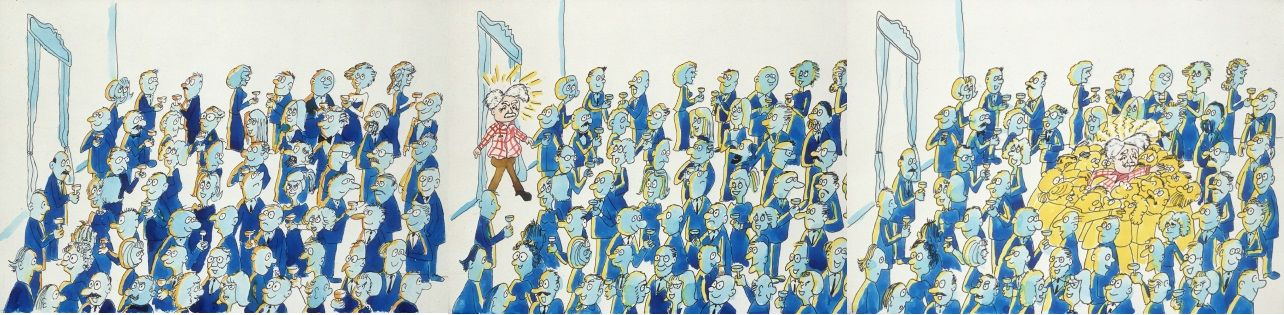
\includegraphics[width=0.9\textwidth,clip] {figures/famousphysicist.jpg}
% \caption{}
% \label{fig:famousphysicist}
% \end{figure}


% \begin{figure}[!hbt]
% \centering
% 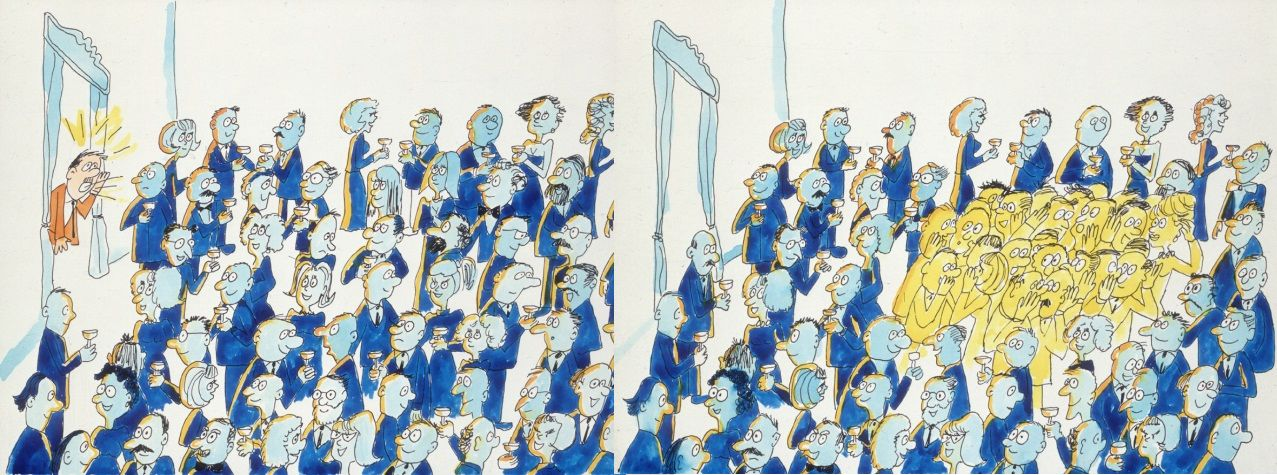
\includegraphics[width=0.9\textwidth,clip] {figures/gossip.jpg}
% \caption{}
% \label{fig:gossip}
% \end{figure}



%====================================================================================================


For decades, the Higgs boson remained the final missing piece of the SM. Its discovery required a collider capable of reaching energy scales high enough to produce it. This challenge was met by the Large Hadron Collider (LHC) at CERN, where the ATLAS and CMS experiments, in 2012, independently observed a particle consistent with the predicted properties of the Higgs boson. This landmark discovery confirmed the Higgs mechanism and earned François Englert and Peter Higgs the 2013 Nobel Prize in Physics.

While the Higgs boson’s discovery marked a triumph for the SM, it also highlighted unresolved mysteries in fundamental physics. Among the persistent shortcomings of the SM, we note that there is no inclusion of a force carrier for gravity, or so-called ``graviton.'' Furthermore, the SM still does not contain any description of dark matter, which seems to outweigh visible matter roughly six to one. Or any explanation for the matter-antimatter asymmetry that we observe in our universe, despite the fact that, in principle, particles formed in the early universe should have had an equal chance of becoming matter or antimatter.
%~\cite{Darkmatt18}%~\cite{Thematte44}

Answers to these questions, or at least hints to guide our way, hinge upon the search for evidence of physics Beyond the Standard Model (BSM). Given the extraordinary success of the SM in describing the known fundamental particles and their interactions, any necessary modifications or extensions to this framework are most effectively probed through the observation of subtle anomalies, discrepancies between theoretical expectations and precision measurements. The Higgs boson offers a natural point of connection to potential new physics, particularly in the context of dark matter\footnote{Dark matter remains elusive, with its non-gravitational interactions yet to be directly detected.}. Since dark matter must possess mass to interact gravitationally, it is plausible that dark matter particles couple to the Higgs boson.
%~\cite{CERNandt20}

If dark matter (or any other anomalous particle) does indeed couple to the Higgs field, then precise measurements of Higgs boson production and decay processes could reveal subtle anomalies—shifts in branching ratios, invisible decays, or unexpected interaction strengths—that point toward the existence of new, BSM particles. Thus, studying the Higgs boson in unprecedented detail represents one of our most promising strategies for uncovering the true nature of dark matter and extending our understanding of fundamental physics beyond the SM.



% Answers to these questions or at least hints to guide our way, we expect to find through evidence of BSM (Beyond the Standard Model) physics. Necessary changes or extensions to the SM framework are likely best probed through the observation of anomalous behavior, or physics that does not exactly match our Standard Model predictions. And with the (relatively) recent experimental confirmation of the Higgs boson, we now have a promising window through which we can search for such anomalous behavior. Because of the role that the Higgs field plays in giving mass to particles through the Brout-Englert-Higgs mechanism, it is reasonable to expect dark matter particles to exhibit some coupling to the Higgs boson~\cite{CERNandt20}. In fact, because dark matter seems to strictly interact with observable matter through gravitational effects, probing at the mechanism which gives it mass may be our best way to learn more about its characteristics.


% Extensions of the Standard Model, such as supersymmetry and grand unified theories, propose new particles and interactions that could address these open questions. Experimental searches at high-energy colliders, neutrino observatories, and astrophysical experiments continue to probe these mysteries, potentially paving the way for the next major breakthrough in our understanding of fundamental physics.

% The Higgs mechanism, once a theoretical curiosity, has become a central pillar of modern physics. From its conceptual origins in superconductivity to its incorporation into the electroweak theory and its experimental confirmation, the Higgs field has reshaped our understanding of mass, symmetry breaking, and fundamental forces. Yet, despite its success, many questions remain unanswered, ensuring that the quest for deeper insights into the nature of the universe continues.

%====================================================================================================

% The Standard Model includes 4 force carriers: the gluon, photon, Z boson, and W boson. These mediate the strong, electromagnetic, and weak forces respectively. The discovery of the Higgs boson in 2012 at the Large Hadron Collider (LHC) added a significant contribution to this picture of our physical understanding, via an experimentally confirmed Higgs field with which various elementary particles can interact to acquire mass. 

% Among the persistent shortcomings of the Standard Model, we note that there is no inclusion of a force carrier for gravity, or so-called ``graviton.'' Furthermore, the Standard Model still does not contain any description of dark matter, which seems to outweigh visible matter roughly six to one~\cite{Darkmatt18}. Or any way to explain the matter/antimatter asymmetry that we observe in our universe where matter is abundant, despite the fact that in principle, after the Big Bang, particles formed in the early universe should have had an equal chance of becoming matter or antimatter~\cite{Thematte44}.

% Answers to these questions or at least hints to guide our way, we expect to find through evidence of BSM (Beyond the Standard Model) physics, essentially extensions to our current Standard Model. While it is possible that our description of elementary physics will require an overhaul in the future, the consistent reliability of the Standard Model provides a promising starting point and very accurate physical description at the energies that we can experimentally observe as a species.

% Such necessary changes to the SM framework are likely best probed through the observation of anomalous behavior, or physics that does not exactly match our Standard Model predictions. And with the (relatively) recent experimental confirmation of the Higgs boson, we now have a promising window through which we can search for such anomalous behavior. Because of the role that the Higgs field plays in giving mass to particles through the Brout-Englert-Higgs mechanism, it is reasonable to expect dark matter particles to exhibit some coupling to the Higgs boson~\cite{CERNandt20}. In fact, because dark matter seems to strictly interact with observable matter through gravitational effects, probing at the mechanism which gives it mass may be our best way to learn more about its characteristics.









\section{Phenomenology of the off-shell Higgs boson}


% % epigraph after chapter heading
% \epigraph{Since it is written in \LaTeX, it must be true.}{-- Isaac Newton}


%%%% MUST: add the citation for the chapter if it is a reprint

% \blindtext\footnote{Hello, this is the first footnote with no indentation and single-spaced text. The spacing between two footnotes is also single-spaced.}

Since 2012, both ATLAS and CMS have observed a Higgs Boson with mass around 125 GeV~\cite{20121}~\cite{201230} which is consistent with our SM expectations. The Higgs boson's mass, as the last free parameter of the SM, is necessarily determined experimentally and is instrumental in our understanding of the SM, along with the Higgs boson's other properties such as its width and couplings to other particles. This is because the Higgs mass relies on the value of $\lambda$ as seen in \ref{eq:higgpot}, an a priori unknown free parameter. It is also tied to the value of the Higgs width and $\mu^2$. Ergo, any precision measurements of the Higgs boson are invaluable in our search for deviations from our SM expectation.

% For every interaction the Higgs has with a fermion, there’s a unique coupling constant which determines the mass of that particle. But it also helps us calculate the rate of decay of the Higgs into other particles. 

Now, in the SM, ``virtual'' particles can have a mass that is different from the mass that the
particle would have if it were ``real,'' or physical. Inside a Feynman diagram\footnote{Feynman diagrams are pictorial representations of interactions between subatomic particles. They provide an intuitive way to illustrate and organize the many terms which arise in expansions of quantum field theory (QFT) descriptions of such interactions.}, virtual particles can have any mass because they aren’t physical, stable particles; they are excitations in quantum fields. This lets us draw Feynman diagrams with intermediary particles of masses very different from their SM mass. An example of this is illustrated in Figure~\ref{fig.Hdecay} in which a Higgs boson ($m_{H,SM} \approx 125$ GeV) can decay to two physical Z bosons ($2m_{Z,SM} \approx 182$ GeV). The SM mass, also referred to as the ``pole mass'' is the mass value which matches the mathematical pole of each particle's renormalized propagator in momentum space. It can also be thought of as the physical mass of the particle as observed, for example if measured in scattering experiments.

We call particles with masses away from their pole mass ``off-shell.''  This terminology arises from the notion that a particle is produced ``on the mass shell'' when its invariant mass\footnote{Note that the invariant mass is a Lorentz-invariant quantity defined from a particle's four-momentum, and includes both energy and momentum such that it remains constant regardless of boost or frame. For on-shell particles, this coincides with the rest mass.} matches the SM expectation, whereas an ``off the mass shell'' particle is produced with invariant mass higher or lower than its nominal pole mass. This thesis will focus on measurements of the off-shell Higgs boson, for reasons to be presented. 

\subsection{Production Modes}

At collision energies around 13 TeV, we certainly have enough energy to produce the Higgs boson at the LHC, as observed in the plot of proton-proton cross sections in Figure~\ref{fig:prodModes}. To provide a sense of scale, assuming SM cross sections, $\sim1$ Higgs bosons are produced every second. Further details are presented in Section~\ref{chap:LHC}.

Production occurs via four dominant modes which have the Feynman diagrams illustrated in Figure~\ref{fig.Hproduction}. As one can see, each of the dominant production diagrams begin with quarks or gluons from the proton-proton collisions. Our dominant production mode, gluon fusion, can be seen in Figure~\ref{fig.ggH} and at leading order involves a quark loop since the Higgs boson does not couple directly to the massless gluons. The primary contribution is with a loop of top quarks (the heaviest quark), with a small contribution from the bottom quark (the second heaviest). At higher order, radiated gluons and other jets (created through QCD effects from the inital state gluons) can be produced along with the Higgs boson. 

The second most productive mechanism is vector boson fusion (VBF), shown in Figure~\ref{fig.VBF}, in which two vector bosons are radiated from our initial state quarks and then interact to ``fuse'' and generate a Higgs boson. Because the W and Z vector bosons have mass around 80-90 GeV, VBF can involve the radiation of hundreds of GeV especially at higher energies when the vector bosons come on-shell. This means that the two quark jets emitted from a VBF event characteristically possess large transverse energies and are often emitted opposite each other. 

\begin{figure}[!hbt]
\centering
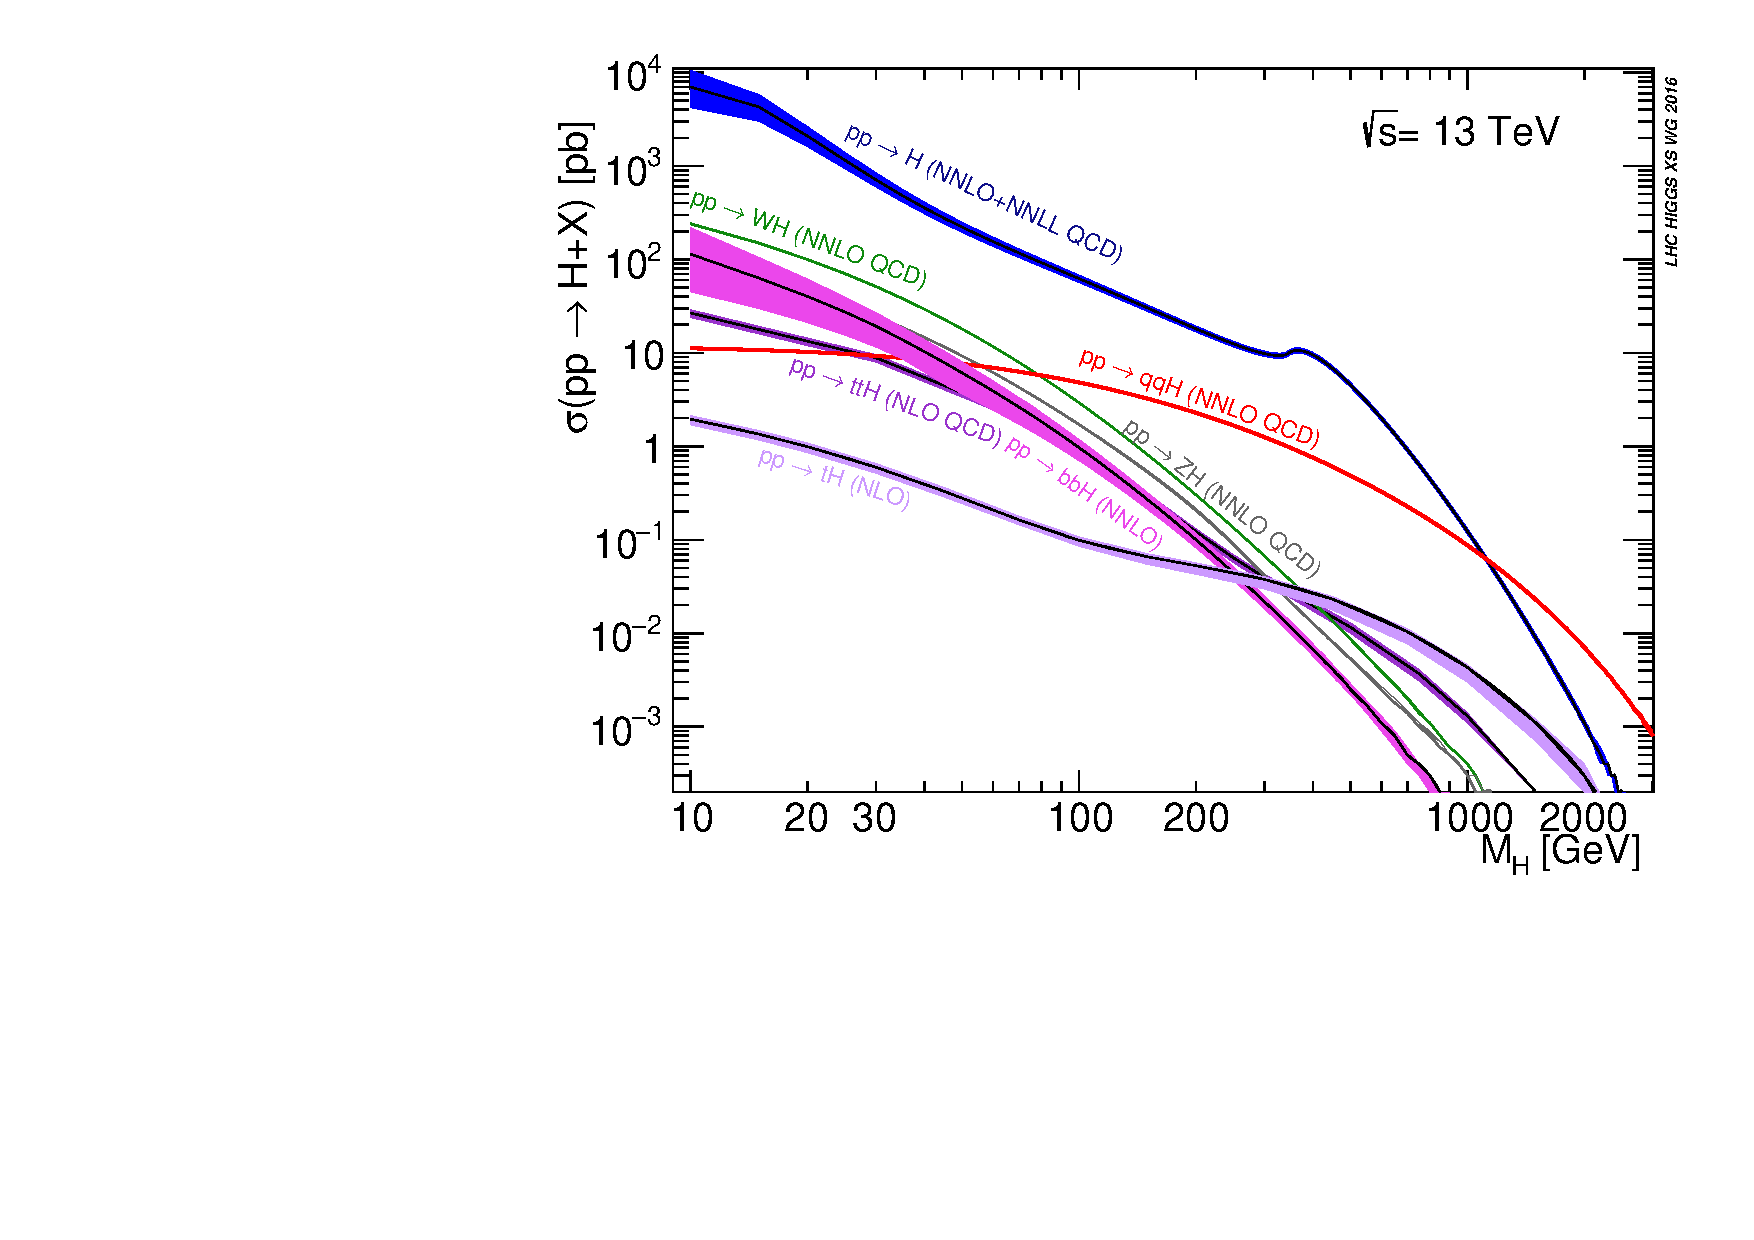
\includegraphics[width=0.75\textwidth,clip] {figures/plotAll_13tev_BSM_sqrt.pdf}
\caption{SM Higgs boson production cross sections as a function of $m_{H}$ at the LHC at $E_{CM}=13$ TeV~\cite{YR4}.}
\label{fig:prodModes}
\end{figure}

The third most common production mode for both on-shell and off-shell Higgs boson production is associated production with a vector boson, or VH production. This is also known as Higgs-strahlung production, since it closely resembles how a photon can be radiated by an electron through Bremsstrahlung radiation. In VH production, as seen in Figure \ref{fig.VH}, two initial state quarks will produce an energetic vector boson which radiates a Higgs boson. Such that a q$\bar{\text{q}}$ initial state results in a VH final state. 

Finally, most of the remaining Higgs boson cross section comes from ttH production, Figure \ref{fig.ttH}. This production mode, along with bbH and other less common mechanisms, becomes less relevant in the production of the off-shell Higgs boson as one can see in Figure \ref{fig:prodModes}. In the off-shell region (chosen to include energies above 220 GeV), the relevant production modes to consider are ggH, VBF, and VH. 

\begin{figure}[!hbt]\centering
\vspace{7mm}
    \begin{subfigure}{0.4\textwidth}
        \begin{fmffile}{ggH}
          \begin{fmfgraph*}(150,80)
            \fmfstraight
            \fmfleft{i1,i2}
            \fmfright{o1,m,o2}
            % gluons
            \fmf{gluon}{i1,t1}
            \fmf{gluon}{t2,i2}
            \fmf{phantom,tension=0.4}{t1,o1}
            \fmf{phantom,tension=0.4}{t2,o2}
            \fmffreeze
            % top loop
            \fmf{fermion,tension=1}{t1,t2,t3,t1}
            \fmf{phantom,tension=1.4}{t3,m}
            \fmffreeze
            % Higgs boson
            % \fmf{dashes,tension=1.4}{t2,h}
            \fmf{dashes,tension=1.4}{t3,m}
            % \fmf{dashes,tension=1}{h,o2}
            \fmflabel{$g$}{i1}
            \fmflabel{$g$}{i2}
            \fmflabel{H}{m}
            % \fmf{dashes,tension=1}{h,o1}
            % \fmf{dashes,tension=1}{h,o2}
          \end{fmfgraph*}
        \end{fmffile}
        \caption{}
        \label{fig.ggH}
    \end{subfigure}
\hfil
    \begin{subfigure}{0.4\textwidth}
        \begin{fmffile}{VBF}
          \begin{fmfgraph*}(150,80)
            \fmfleft{i1,i3} 
            \fmfright{o1,o2,o3}
            \fmf{fermion}{i1,v1,o1}
            \fmf{fermion}{i3,v3,o3}
            \fmf{phantom,tension=0.3}{v1,v3}
            \fmffreeze
            \fmf{boson,label=$V$,label.side=left}{v3,v2,v1}
            \fmf{boson}{v3,v2,v1}
            \fmf{dashes}{v2,o2}
            \fmflabel{$q$}{o1}
            \fmflabel{$q$}{o3}
            \fmflabel{$q$}{i3}
            \fmflabel{$q$}{i1}
            \fmflabel{H}{o2}
          \end{fmfgraph*}
        \end{fmffile}
        \caption{}
        \label{fig.VBF}
    \end{subfigure}
\hfil
\vspace{7mm}
    \begin{subfigure}{0.4\textwidth}
        \begin{fmffile}{VH}
          \begin{fmfgraph*}(150,80)
            \fmfset{wiggly_len}{18}
            \fmfleft{i1,i2}
            \fmfright{o1,o2}
            \fmf{fermion}{v1,i1}
            \fmf{fermion}{i2,v1}
            % \fmf{boson,label=$V^*$,label.side=left}{v1,v2}
            \fmf{boson}{v1,v2}
            % \fmf{boson,label.side=left}{v2,o2}
            \fmf{boson}{v2,o2}
            \fmf{dashes}{v2,o1}
            \fmflabel{$q'$}{i1}
            \fmflabel{$q$}{i2}
            \fmflabel{$V$}{o2}
            \fmflabel{H}{o1}
          \end{fmfgraph*}
        \end{fmffile}
    \caption{}
    \label{fig.VH}
    \end{subfigure}
\hfil
    \begin{subfigure}{0.4\textwidth}
        \begin{fmffile}{ttH}
          \begin{fmfgraph*}(150,80)
            \fmfleft{d,i1,d,d,i3,d}
            \fmfright{o1,d,o2,d,o3}
            \fmf{gluon,tension=1.2}{i1,v1}
            \fmf{gluon,tension=1.2}{v3,i3}
            \fmf{fermion}{o1,v1}
            \fmf{fermion}{v3,o3}
            \fmf{phantom,tension=0.3}{v1,v3}
            \fmffreeze
            \fmf{fermion}{v1,v2,v3}
            \fmf{dashes,tension=1.3}{v2,o2}
            \fmflabel{$g$}{i3}
            \fmflabel{$g$}{i1}
            \fmflabel{$t$}{o3}
            \fmflabel{$\bar{t}$}{o1}
            \fmflabel{H}{o2}
          \end{fmfgraph*}
        \end{fmffile}
    \caption{}
    \label{fig.ttH}
    \end{subfigure}
    \caption{Feynman diagrams for the dominant Higgs boson production modes at the LHC: (a) gluon fusion (ggH), (b) vector boson fusion (VBF), (c) associated (VH) production, and (d) t$\bar{\text{t}}$H production.}
    \label{fig.Hproduction}
\end{figure}

\subsection{Decay Modes}

% The Higgs boson couples to its decay products based on their masses. At a Higgs mass of 125 GeV or lower, the dominant decay mode is H $\rightarrow$ bb, as b-quarks are the heaviest available decay products. At higher masses, the decays H $\rightarrow$ WW and H $\rightarrow$ ZZ become more prevalent. Relative to the vector boson decays, the channels H $\rightarrow$ $\gamma \gamma$ and H $\rightarrow$ Z$\gamma$ have significantly smaller branching ratios because a massless photon cannot couple directly to the Higgs, and thus requires a loop with massive particles to mediate.

% The sensitivity of a particular decay channel depends on its branching ratio, reconstructed mass resolution, and backgrounds. The H $\rightarrow$ bb channel faces significant QCD background noise and has poor mass resolution. In the H $\rightarrow$ WW channel, missing energy from neutrinos in the final decay products can complicate detection of Higgs events. So, although its expected cross section is smaller compared to H $\rightarrow$ bb or H $\rightarrow$ WW, the H $\rightarrow$ ZZ $\rightarrow$ 4l process has minimal background interference and allows for full decay kinematics with high resolution. This is why the H $\rightarrow$ ZZ $\rightarrow$ 4l is often also referred to as the ``Golden Channel'' and is an ideal channel for both the discovery and measurement of the Higgs boson's properties.

The interaction strength of the Higgs boson with its decay products is directly proportional to their masses. As illustrated in Figure \ref{fig:HiggsBR}, at a Higgs boson mass around 125 GeV, the dominant decay mode is \( H \to b\bar{b} \), since the bottom quark is the heaviest kinematically accessible fermion. However, as the Higgs boson's mass increases beyond this threshold, decays into electroweak gauge bosons, specifically \( H \to WW \) and \( H \to ZZ \), become dominant due to their larger coupling strength and enhanced phase space availability as there is enough energy for the vector bosons to exist on-shell. The loop-induced processes \( H \to \gamma\gamma \) and \( H \to Z\gamma \) have significantly lower branching fractions, as the Higgs boson does not couple directly to massless photons; these decays proceed via higher-order quantum corrections involving virtual heavy particles in the loop, such as top quarks or W bosons.

\begin{figure}[!hbt]
\centering
\begin{subfigure}[t]{0.45\textwidth}
    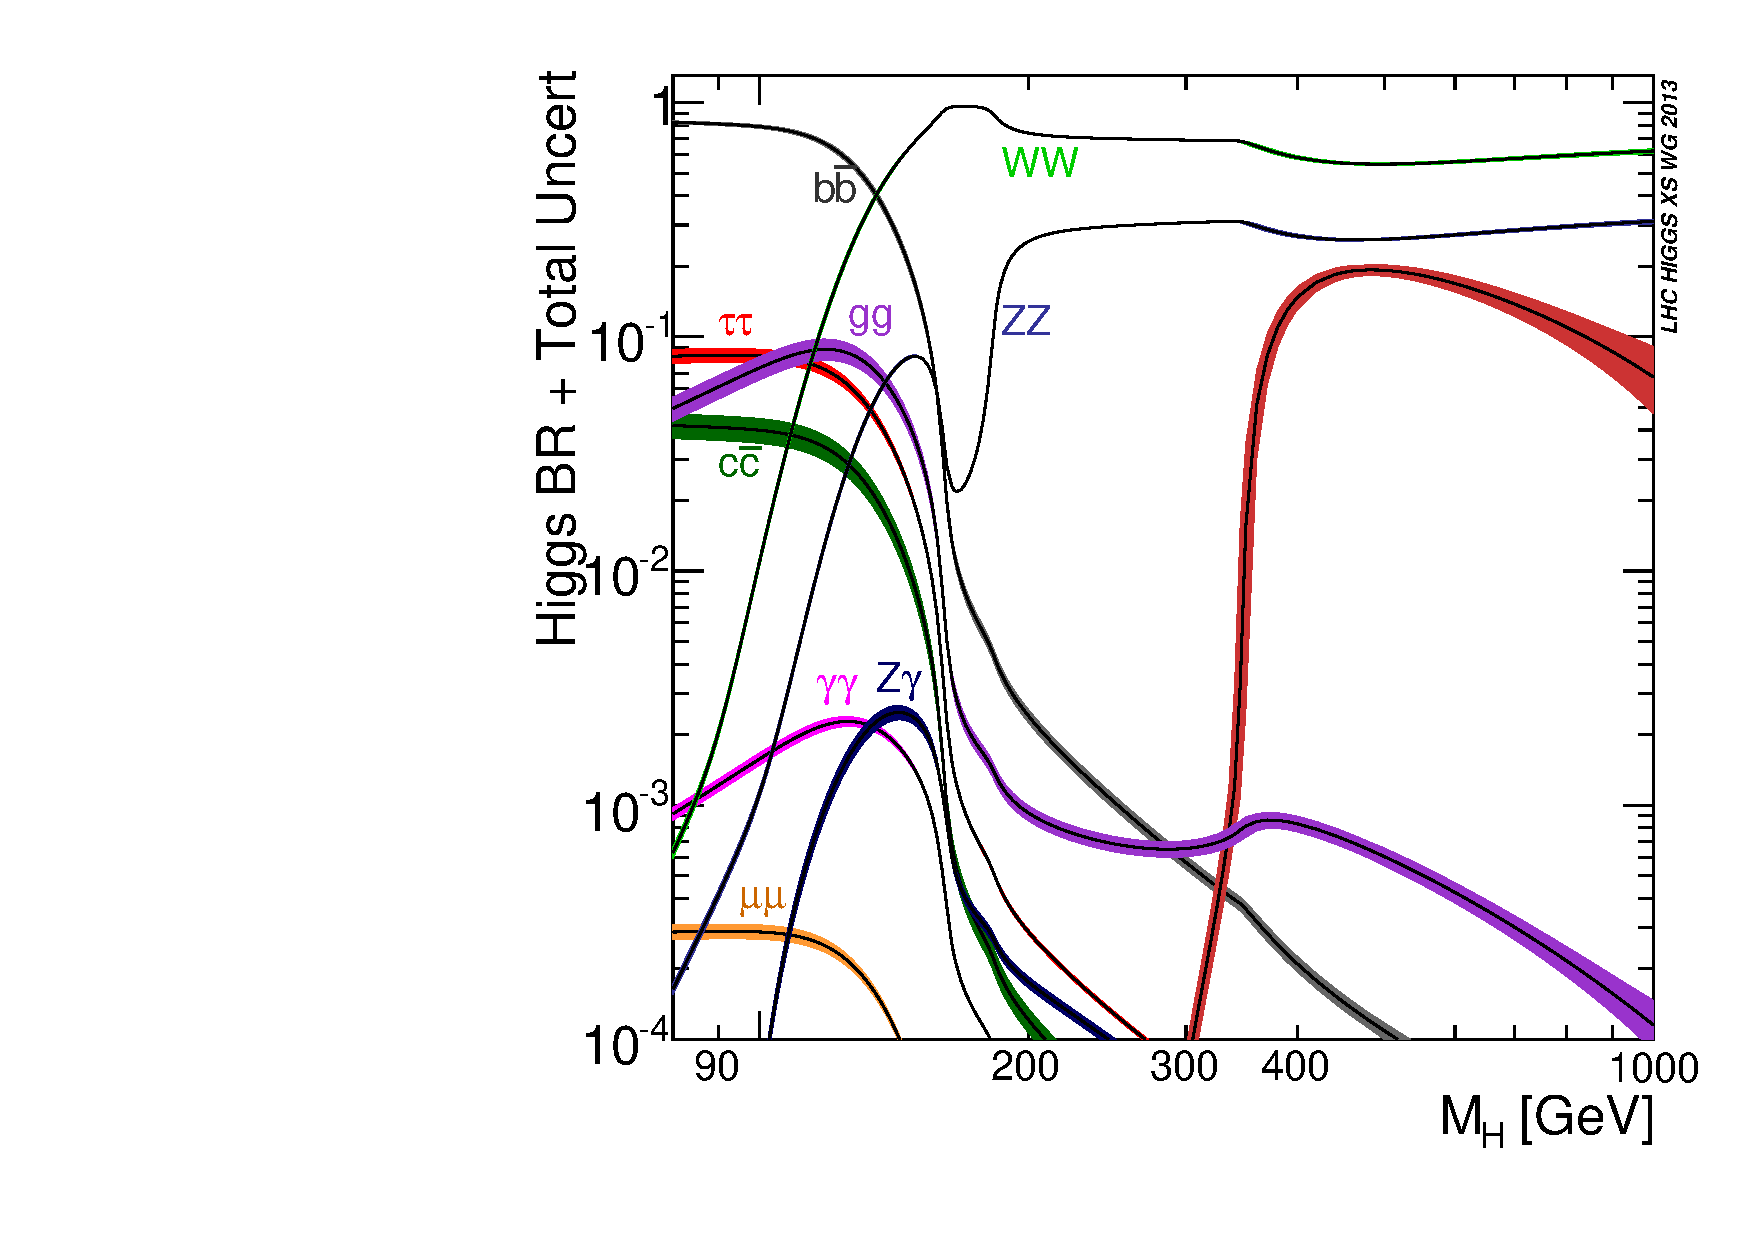
\includegraphics[width=\textwidth]{figures/Higgs_BR.pdf}
    \caption{}
    \label{fig:HiggsBR}
\end{subfigure}
\begin{subfigure}[t]{0.45\textwidth}
    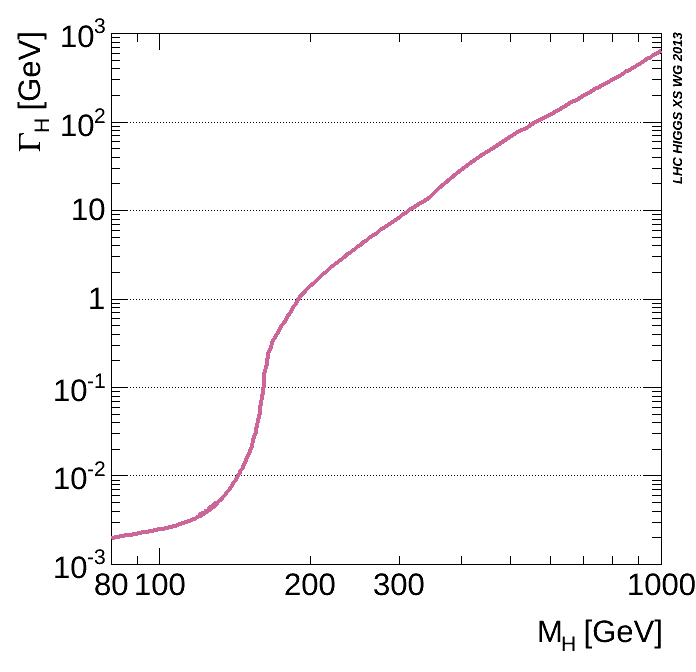
\includegraphics[width=\textwidth]{figures/SM_Width.png}
    \caption{}
    \label{fig:SMwidth}
\end{subfigure}
\caption{SM Higgs boson decay branching ratios (a) and total decay width (b) as a function of mass $m_{H}$~\cite{YR4}. In the off-shell region above 220 GeV, the Higgs boson decay to a pair of vector bosons dominates. We see an enhancement of the Higgs boson width at energies above $2m_V$ when the two vector bosons become on-shell.}
\label{fig:HiggsDecay}
\end{figure}

The experimental sensitivity of a given decay channel is determined not only by the branching fraction but also by factors such as the mass resolution of reconstructed final states and the level of irreducible and reducible backgrounds. The \( H \to b\bar{b} \) channel, despite its large branching ratio, suffers from overwhelming quantum chromodynamic (QCD) backgrounds and poor mass resolution, making precise measurements challenging. The \( H \to WW \) decay, while more distinctive, involves final-state neutrinos that escape detection, leading to missing transverse energy and complications in fully reconstructing the Higgs boson's invariant mass.

% The \( H \to ZZ \) channel, although having a smaller overall production cross section compared to \( H \to b\bar{b} \) or \( H \to WW \), 
The \( H \to ZZ \) channel provides a particularly clean final state, especially in the fully leptonic decay mode \( H \to ZZ \to 4\ell \) (where \( \ell = e, \mu \)). This process benefits from a low background contamination, fully reconstructible decay products, and excellent mass resolution, making it an optimal channel for precision measurements of the Higgs boson properties. As a result, this thesis will primarily focus on the \( H \to ZZ \) decay mode for detailed studies of the Higgs boson, as visualized in Figure~\ref{fig.Hdecay}.

% \begin{figure}[!hbt]\centering
%     \begin{fmffile}{decay}
%       \begin{fmfgraph}(170,150)
%         \fmfstraight
%         \fmfleft{i0,i1,i2}
%         \fmfright{o1,o2,o3,o4}
%         % fermions
%         \fmf{fermion}{o1,v21,o2}
%         \fmf{fermion}{o3,v22,o4}
%         % phantoms to pull back fermion lines
%         \fmf{phantom}{i0,v21}
%         \fmf{phantom,tension=0.5}{v21,v22}
%         \fmf{phantom}{i2,v22}
%         \fmffreeze
%         % HWW
%         \fmf{dashes,tension=1.5}{i1,v1}
%         \fmf{boson}{v1,v21}
%         \fmf{boson}{v1,v22}
%       \end{fmfgraph}
%     \end{fmffile}
%     \caption{Feynman diagram for the decay of a Higgs boson to two vector bosons and four leptons.}
%     \label{fig.Hdecay}
% \end{figure}


\begin{figure}[!hbt]
  \centering
  \begin{tikzpicture}
    \begin{feynman}
      \vertex (h) {\(H^{(*)}\)};
      \vertex [right=3cm of h] (v);
      \vertex [above right=3cm of v] (z1);
      \vertex [below right=3cm of v] (z2);
      
      \vertex [right=3cm of z1] (l1) {\(\ell^-\)};
      \vertex [below=1.5cm of l1] (l2) {\(\ell^+\)};
      
      \vertex [right=3cm of z2] (l3) {\(\ell^-\)};
      \vertex [above=1.5cm of l3] (l4) {\(\ell^+\)};
      
      \diagram* {
        (h) -- [scalar] (v),
        (v) -- [boson, edge label=\(Z\)] (z1),
        (v) -- [boson, edge label=\(Z^{(*)}\)] (z2),
        (z1) -- [fermion] (l1),
        (z1) -- [anti fermion] (l2),
        (z2) -- [fermion] (l3),
        (z2) -- [anti fermion] (l4),
      };
    \end{feynman}
  \end{tikzpicture}
  \caption{Feynman diagram for the decay \(H^{(*)} \to ZZ^{(*)} \to 4\ell\).}
  \label{fig.Hdecay}
\end{figure}



% \begin{figure}
% \centering
% 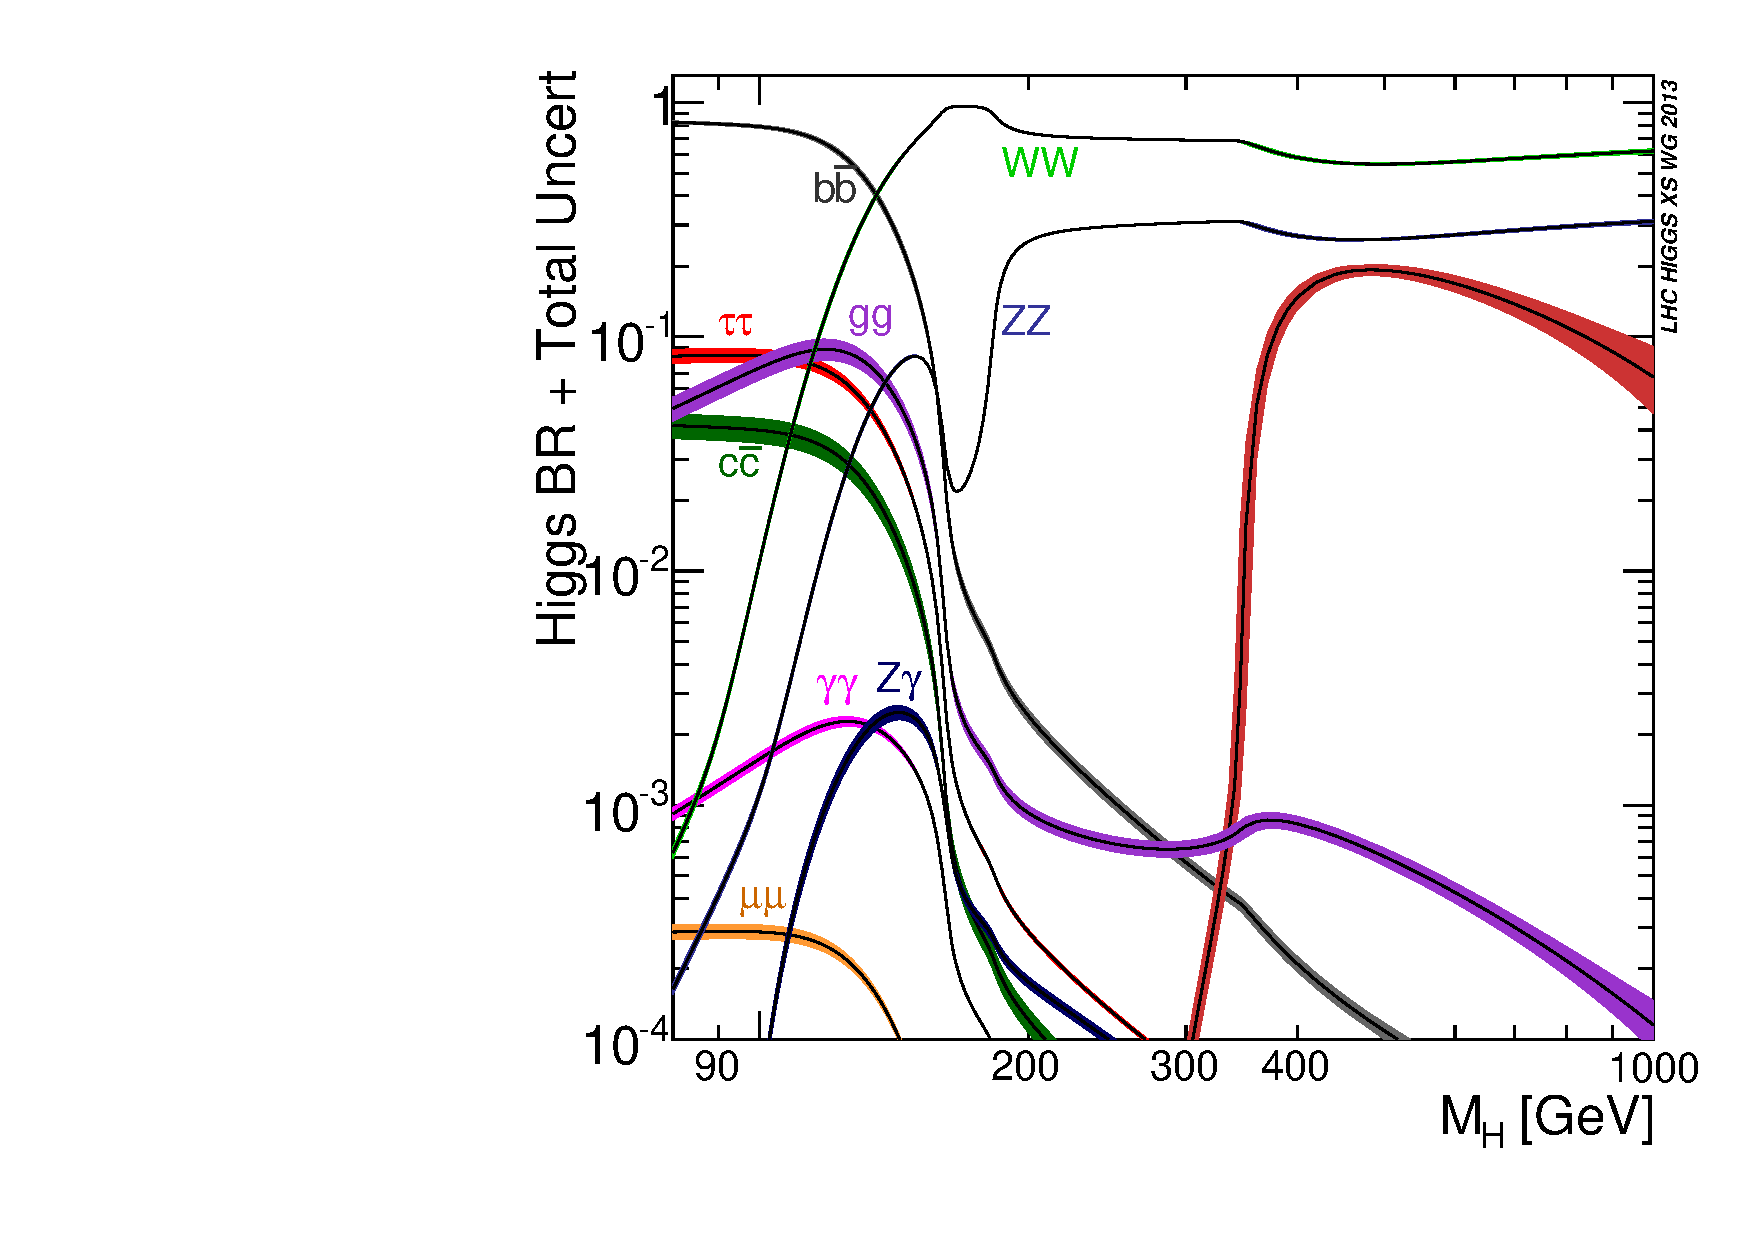
\includegraphics[width=0.8\textwidth,clip] {figures/Higgs_BR.pdf}
% \caption{Standard Model Higgs boson decay branching ratios as a function of mass.}
% \label{fig:HiggsBR}
% \end{figure}

% \begin{figure}
% \centering
% 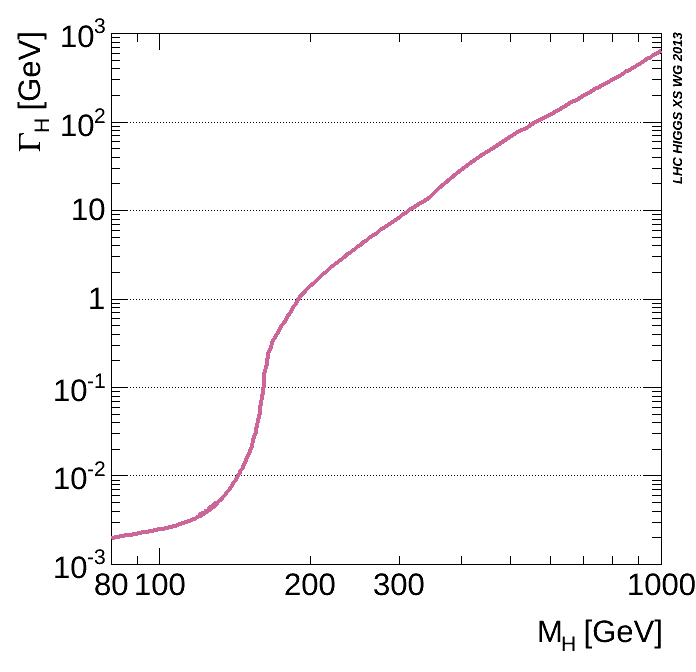
\includegraphics[width=0.8\textwidth,clip] {figures/SM_Width.png}
% \caption{Standard Model Higgs boson total width as a function of mass.}
% \label{fig:SMwidth}
% \end{figure}

\section{Properties of the Higgs boson}

% One method through which we can quantify possible deviations from our SM expectations is through precise measurements of properties of the Higgs. The Higgs boson is an extremely short-lived particle which rapidly decays into other lighter particles. Any such unstable particle has a finite lifetime $\tau$, which through the uncertainty principle is directly correlated to the width $\Gamma$ of its resonance, also interpreted as the uncertainty in its mass. Because the lifetime of a particle is set by its chance of decaying via various modes, the width of the Higgs boson can be influenced by deviations of the boson's couplings to other particles from our SM expectations. Thus precision measurements in the Higgs sector, especially of the Higgs' width, can act as indirect probes of new couplings. 

% For other particles with relatively broad resonances, the particles' width can be directly measured from a Breit–Wigner distribution over mass, which would peak around the particle's nominal mass. However, because the Higgs boson is so short-lived, its width is too narrow to be accurately measured from the line shape of this probability distribution. Even in the so-called ``golden channel'' of Higgs decay via H $\to$ ZZ$^*$ $\to$ $4\ell$ (named for its clean signature and good mass resolution), direct width measurement at the SM peak is limited by experimental resolution to about 1 GeV, far larger than the expected width of the Standard Model Higgs boson of around 4 MeV.

One of the most effective ways to investigate potential deviations from SM predictions is through precise measurements of the properties of the Higgs boson. As an extremely short-lived particle, the Higgs boson rapidly decays into lighter particles, and its finite lifetime \( \tau \) is inherently connected to the width \( \Gamma \) of its resonance via the uncertainty principle, \( \Gamma = \hbar / \tau \). This width can be interpreted as the intrinsic uncertainty in the particle's mass. Since the decay rate of the Higgs boson is dictated by its couplings to other particles, any deviation from SM predictions in these couplings would manifest as an alteration in its total width. Consequently, high-precision studies of the Higgs sector, particularly measurements of \( \Gamma_H \), provide an indirect but highly sensitive probe of BSM physics, including possible exotic decay channels or modifications to Higgs interactions.

For particles with broad resonances, the total width can be extracted directly from the Breit–Wigner line shape, which characterizes the probability distribution of invariant mass around the nominal mass of the particle. However, the Higgs boson presents a unique challenge in this regard. Due to its extremely short lifetime, the corresponding resonance width is remarkably narrow relative to its mass, making direct measurement from the line shape infeasible. Even in the so-called ``golden channel,'' where the Higgs decays via \( H \to ZZ \to 4\ell \) (a channel renowned for its clean experimental signature and excellent mass resolution), the finite detector resolution limits the direct width measurement to an uncertainty of approximately 1 GeV. This is orders of magnitude larger than the predicted SM Higgs boson width of around 4 MeV, rendering a direct determination of \( \Gamma_H \) at the peak practically impossible.

Given these limitations, alternative methods must be employed to infer the Higgs boson's width. One such approach involves off-shell Higgs boson production, where measurements in kinematic regions far from the Higgs boson pole mass can provide indirect sensitivity to its total width. This method separates Higgs boson-mediated and non-resonant background processes, and utilizes the observed yields of Higgs boson events to extract a measurement of \( \Gamma_H \) that is not constrained by detector resolution. The ability to probe the Higgs boson width through such indirect techniques represents a significant contribution to current precision Higgs boson studies in the ongoing search for deviations from the SM and potential new physics.

\section{Off-shell technique} \label{sec:offshelltech}

In this thesis, we employ the ``off-shell technique,'' originally developed by Caola and Melnikov~\cite{13074935} and implemented by the CMS collaboration~\cite{1405345570}, which currently provides the most stringent constraints on the Higgs boson total width. This method exploits Higgs boson production in two distinct kinematic regimes: the ``on-shell'' region, defined in this case within the invariant mass window of 105 to 140 GeV, and the ``off-shell'' region, characterized by Higgs boson candidates exceeding 220 GeV.

\begin{figure}[!hbt]
\centering
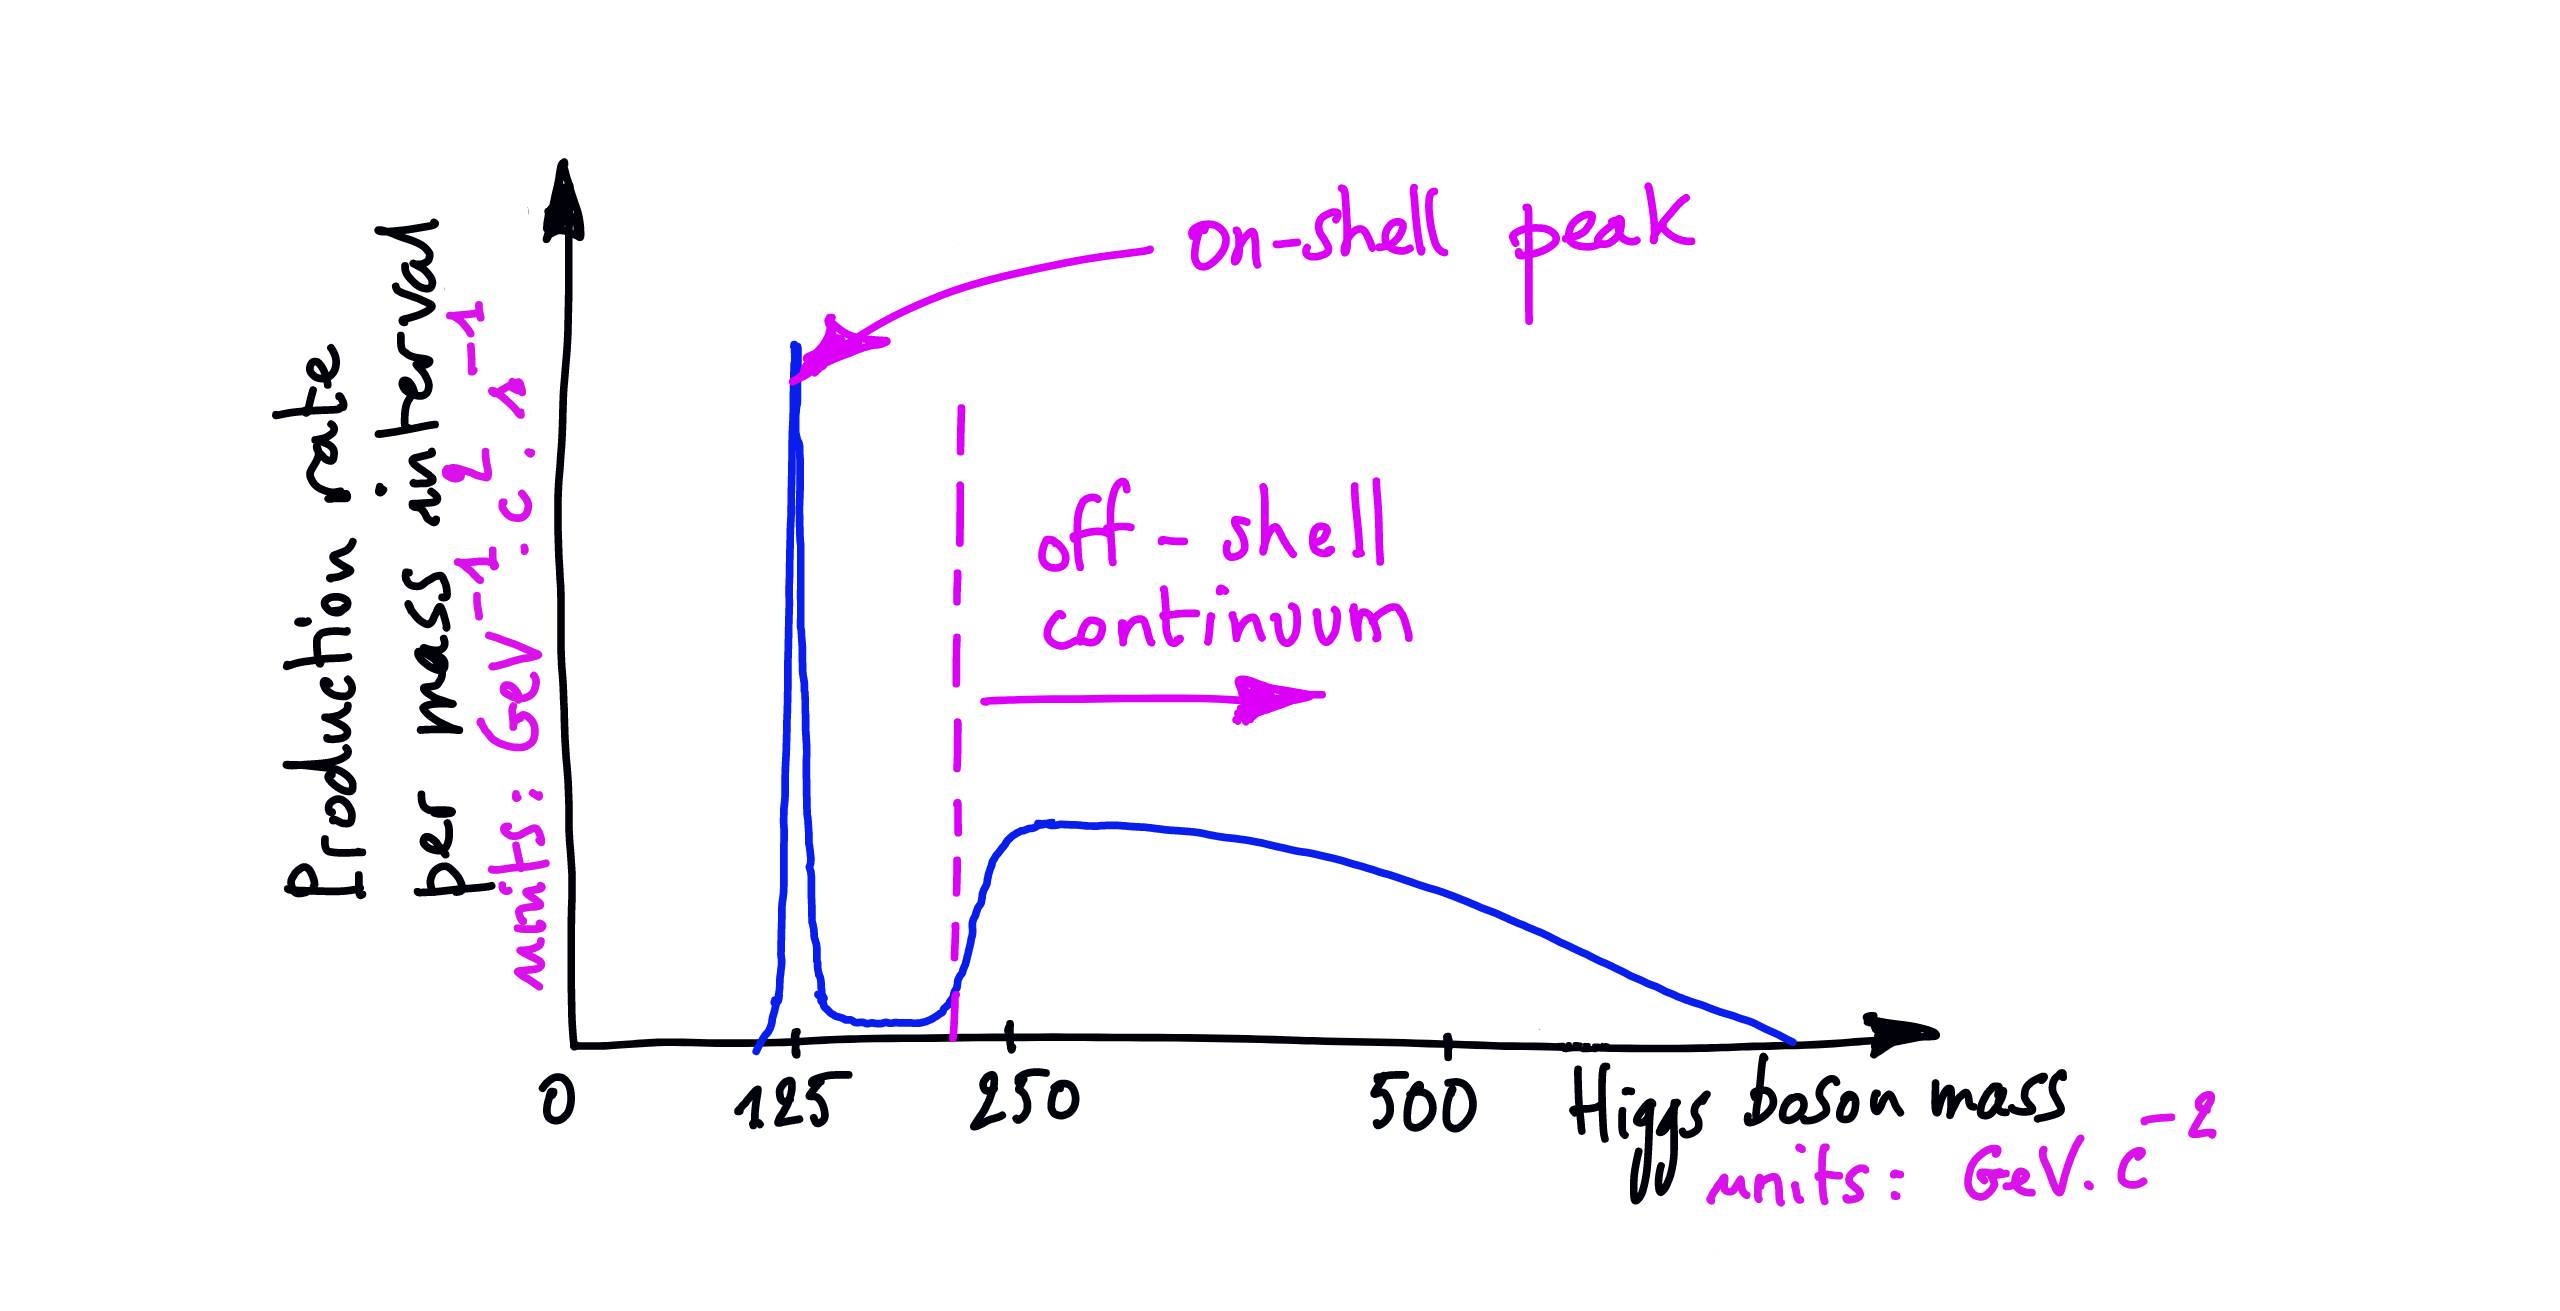
\includegraphics[width=\textwidth,clip] {figures/HIG-21-013_cartoon.png}
\caption{A published sketch of the Higgs boson mass distribution reconstructed from ZZ decays. The peak on the left marks on-shell production while the broad shoulder on the right represents the off-shell process. Beware that the corresponding rates indicated here are not to scale.}
\label{fig:onshelloffshell}
\end{figure}

A seminal study conducted in 2013 by researchers at Johns Hopkins University~\cite{13074935} demonstrated that the total width of the Higgs boson, \( \Gamma_H \), can be inferred by relating the production rates of on-shell and off-shell Higgs bosons. Specifically, by measuring the rate of Higgs production through gluon fusion and subsequent decay via the so-called ``golden channel'' (\( H^* \to ZZ \to 4\ell \)), a direct, resolution-constrained measurement of the Higgs width can be circumvented. Instead, a precise, statistically limited determination of \( \Gamma_H \) is achieved by taking the ratio of off-shell to on-shell Higgs event yields~\cite{190100174}. The proportionalities
\begin{equation}
\label{eq:resonant}
\begin{gathered}
\sigma^\text{on-shell}_{VV \to H \to 4\ell} \propto \mu_{VVH} \frac{1}{\Gamma_H}
\quad\text{and}\quad
\sigma^\text{off-shell}_{VV \to H \to 4\ell} \propto \mu_{VVH},
\end{gathered}
\end{equation}
where \( \mu_{VVH} \) is the signal strength modifier (defined as the ratio of the observed to expected number of on-shell \( 4\ell \) events), give us the relationship
\begin{equation}
\label{eq:widthres}
\begin{gathered}
\Gamma_H \propto \sigma^\text{off-shell}_{VV \to H \to 4\ell} / \sigma^\text{on-shell}_{VV \to H \to 4\ell}.
\end{gathered}
\end{equation}
Since the off-shell to on-shell Higgs boson cross section ratio scales proportionally with \( \Gamma_H \), this method provides a highly sensitive probe of the Higgs boson width.

This approach offers several advantages. In the decay of an on-shell Higgs boson to a pair of massive vector bosons (e.g., ZZ), at least one of the Z bosons must be produced off-shell due to the Higgs boson mass being below the kinematic threshold of \( 2m_Z \approx 180 \) GeV. However, in the off-shell regime (\( m_H > 220 \) GeV), the Higgs boson can decay into two fully on-shell Z bosons, each with a mass of approximately 91 GeV. This results in a significant enhancement\footnote{This enhancement is ``significant'' relative to the dramatic suppression of production as the Higgs boson moves off-shell. Overall, the off-shell range only accounts for $\sim14\%$ of the total number of Higgs boson events.} of the off-shell Higgs production rate at high invariant masses, thereby increasing the available event statistics and improving the precision of the width determination.

Furthermore, the focus on Higgs decays via the \( ZZ \to 4\ell \) channel ensures a clean experimental signature with excellent mass resolution, while also enhancing sensitivity to potential deviations in the Higgs' couplings to vector bosons. As a result, this method not only facilitates a precise measurement of the Higgs boson width but also serves as a robust probe of anomalous contributions to the Higgs–vector boson interaction vertex (HVV). With the LHC operating at a center-of-mass energy of 13.6 TeV in Run 3, the anticipated increase in high-energy collisions will further enhance the statistical power of this technique, enabling even more stringent tests of potential BSM physics.

% In this thesis, we will make use of the ``off-shell technique'' which was developed by CMS~\cite{1405345570} and is currently utilized in order to set the most precise limits on the Higgs boson width. This technique targets Higgs boson production in an ``on-shell'' region between 105 and 140 GeV and in an  ``off-shell'' region defined above 220 GeV. Higgs bosons are said to be produced ``on the mass shell'' if they exist close to the SM mass around 125 GeV and ``off-shell'' if they are produced away from their nominal mass, hence the names for the chosen mass ranges. 

% Through a method proposed by researchers at Hopkins in 2013~\cite{13074935}, it was shown that the width of the Higgs boson can relate the rate of on-shell Higgs boson production to the rate of off-shell production. By counting the number of Higgs bosons produced by strong or electroweak vector bosons ($v$) and that subsequently decay via the golden channel, we can forgo a direct measurement of the Higgs boson width and instead make a very precise width measurement by taking a ratio between the off-shell and on-shell Higgs yields~\cite{190100174}, the relation between which can be described with:
% \begin{equation}
% \label{eq:resonant}
% \begin{gathered}
% \sigma^\text{on-shell}_{vv \to H \to 4\ell} \propto \mu_{vvH}
% \quad\text{and}\quad
% \sigma^\text{off-shell}_{vv \to H \to 4\ell} \propto \mu_{vvH} \Gamma_H,
% \end{gathered}
% \end{equation}
% where $\mu_{vvH}$ is the ratio of the observed to expected number of on-shell $4\ell$ events.

% This approach comes with a few benefits. In the decay of an on-shell Higgs boson to two massive vector bosons (Z for example), one of the Z's must go off-shell since the SM Higgs boson mass is less than twice that of the Z boson. But for an off-shell Higgs with mass above 220 GeV, it is possible to decay via two on-shell Z bosons, each with mass around 90 GeV. Resultantly, we see an enhancement in the rate of Higgs boson production in our off-shell region at energies above what is required for vector boson pair production. This gives us significantly more statistics in our off-shell yield with which to make a precise width measurement. 

% Furthermore, because we are focusing on the Higgs decay via ZZ $\to$ $ 4\ell$, events in this off-shell region are very sensitive to variations in the Higgs' couplings to vector bosons. This means that while making a precise measurement of the Higgs boson width, we can indirectly probe at anomalous terms in the HVV amplitude. (And with the LHC targeting 13.6 TeV collisions in Run 3, we will have even more high-energy events at our disposal in the future.)

% ################################################################################################################

% \begin{figure}
% \centering
% 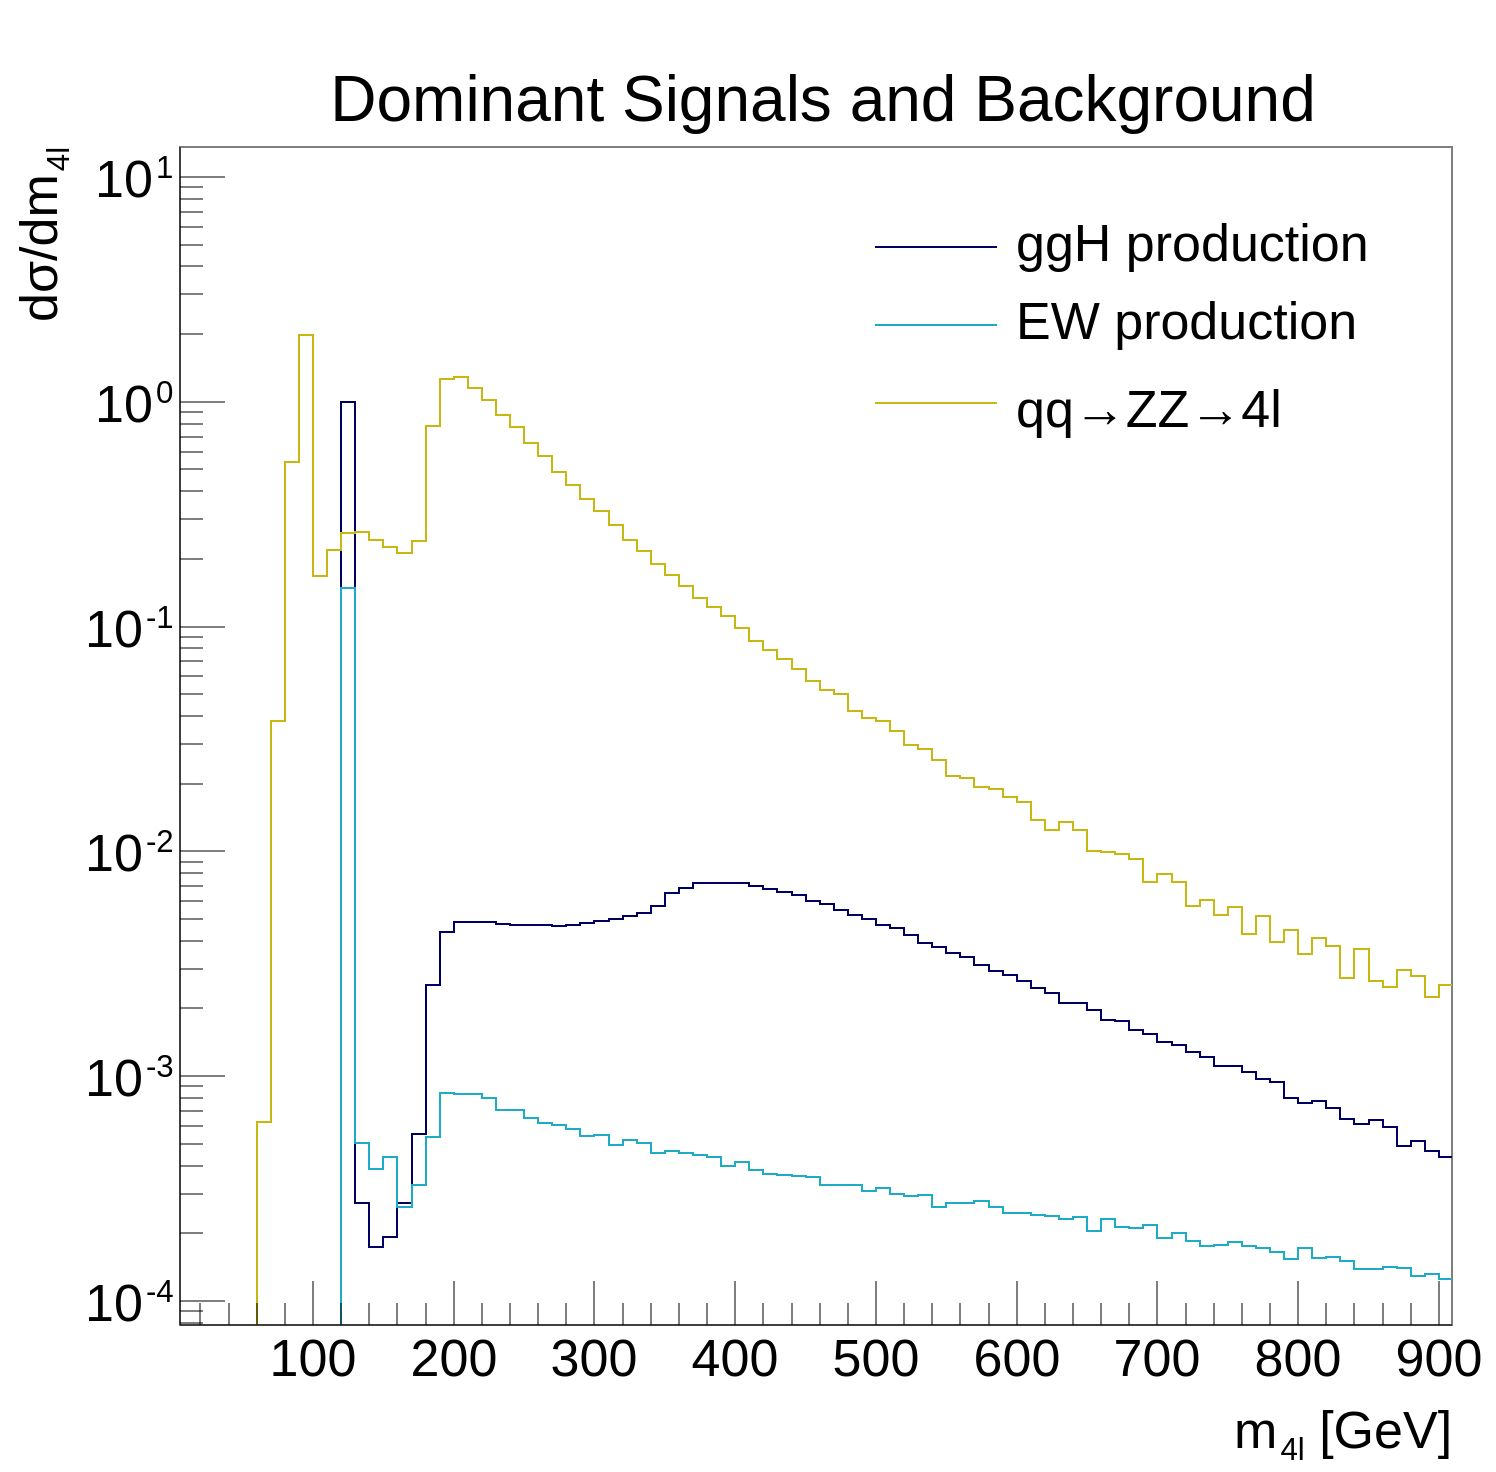
\includegraphics[width=0.8\textwidth,clip] {figures/offshell.jpg}
% \caption{}
% \label{fig:offshell}
% \end{figure}

% \subsection{Composite Higgs Boson}

\section{Higgs Boson Couplings}

In the SM, the Higgs boson couples to gluons via quark loops with Yukawa interactions, where the dominant contribution arises from the top-quark loop, as illustrated in Figure \ref{fig.ggH}. But BSM physics could allow for contributions from new heavy particles in this loop. %~\cite{Gonzalez-Alonso:2014eva,Greljo:2015sla}. 
Yukawa couplings also govern direct interactions with fermion-antifermion pairs, such as in t$\bar{\text{t}}$H and b$\bar{\text{b}}$H production. These interactions are less relevant at high energies due to their suppression, shown in Figure \ref{fig:prodModes}, but they are included in the analysis of on-shell Higgs production under similar assumptions as for gluon fusion.

The Higgs boson couples to the electroweak vector bosons in HVV vertices, without the need for quark mediators. Since we are targeting off-shell Higgs boson production, we have one such vertex on the production sides of two of our primary Feynman diagrams, VBF and VH. And because of our focus on the \( H \to ZZ \) decay channel, we have additional HVV vertices in all of our Feynman diagrams on the decay side. This makes us particularly sensitive to the HVV amplitude overall, which we can use to our advantage.

Beyond the Higgs boson couplings to SM particles, we can also incorporate anomalous coupling strength terms which can be constrained to develop Effective Field Theory (EFT) descriptions. Some examples of familiar vertices in Feynman diagrams that can feature anomalous EFT contributions are shown in Figure \ref{fig:EFTdiagrams}. The anomalous contributions are treated as deviations in the Higgs boson's interactions with two gauge bosons. These anomalous couplings can manifest in both Higgs boson production and decay, regardless of the invariant mass at which the Higgs boson is produced. 
% Equation \ref{eq:resonant} is therefore meant to imply the simultaneous modifications of the $vvH$ couplings in both the on-shell and off-shell regions.
% The anomalous contributions are treated as deviations in the Higgs boson's interactions with two gauge bosons, including $WW, ZZ, Z\gamma, \gamma\gamma$, and $gg$.

\begin{figure}[!hbt]
\centering
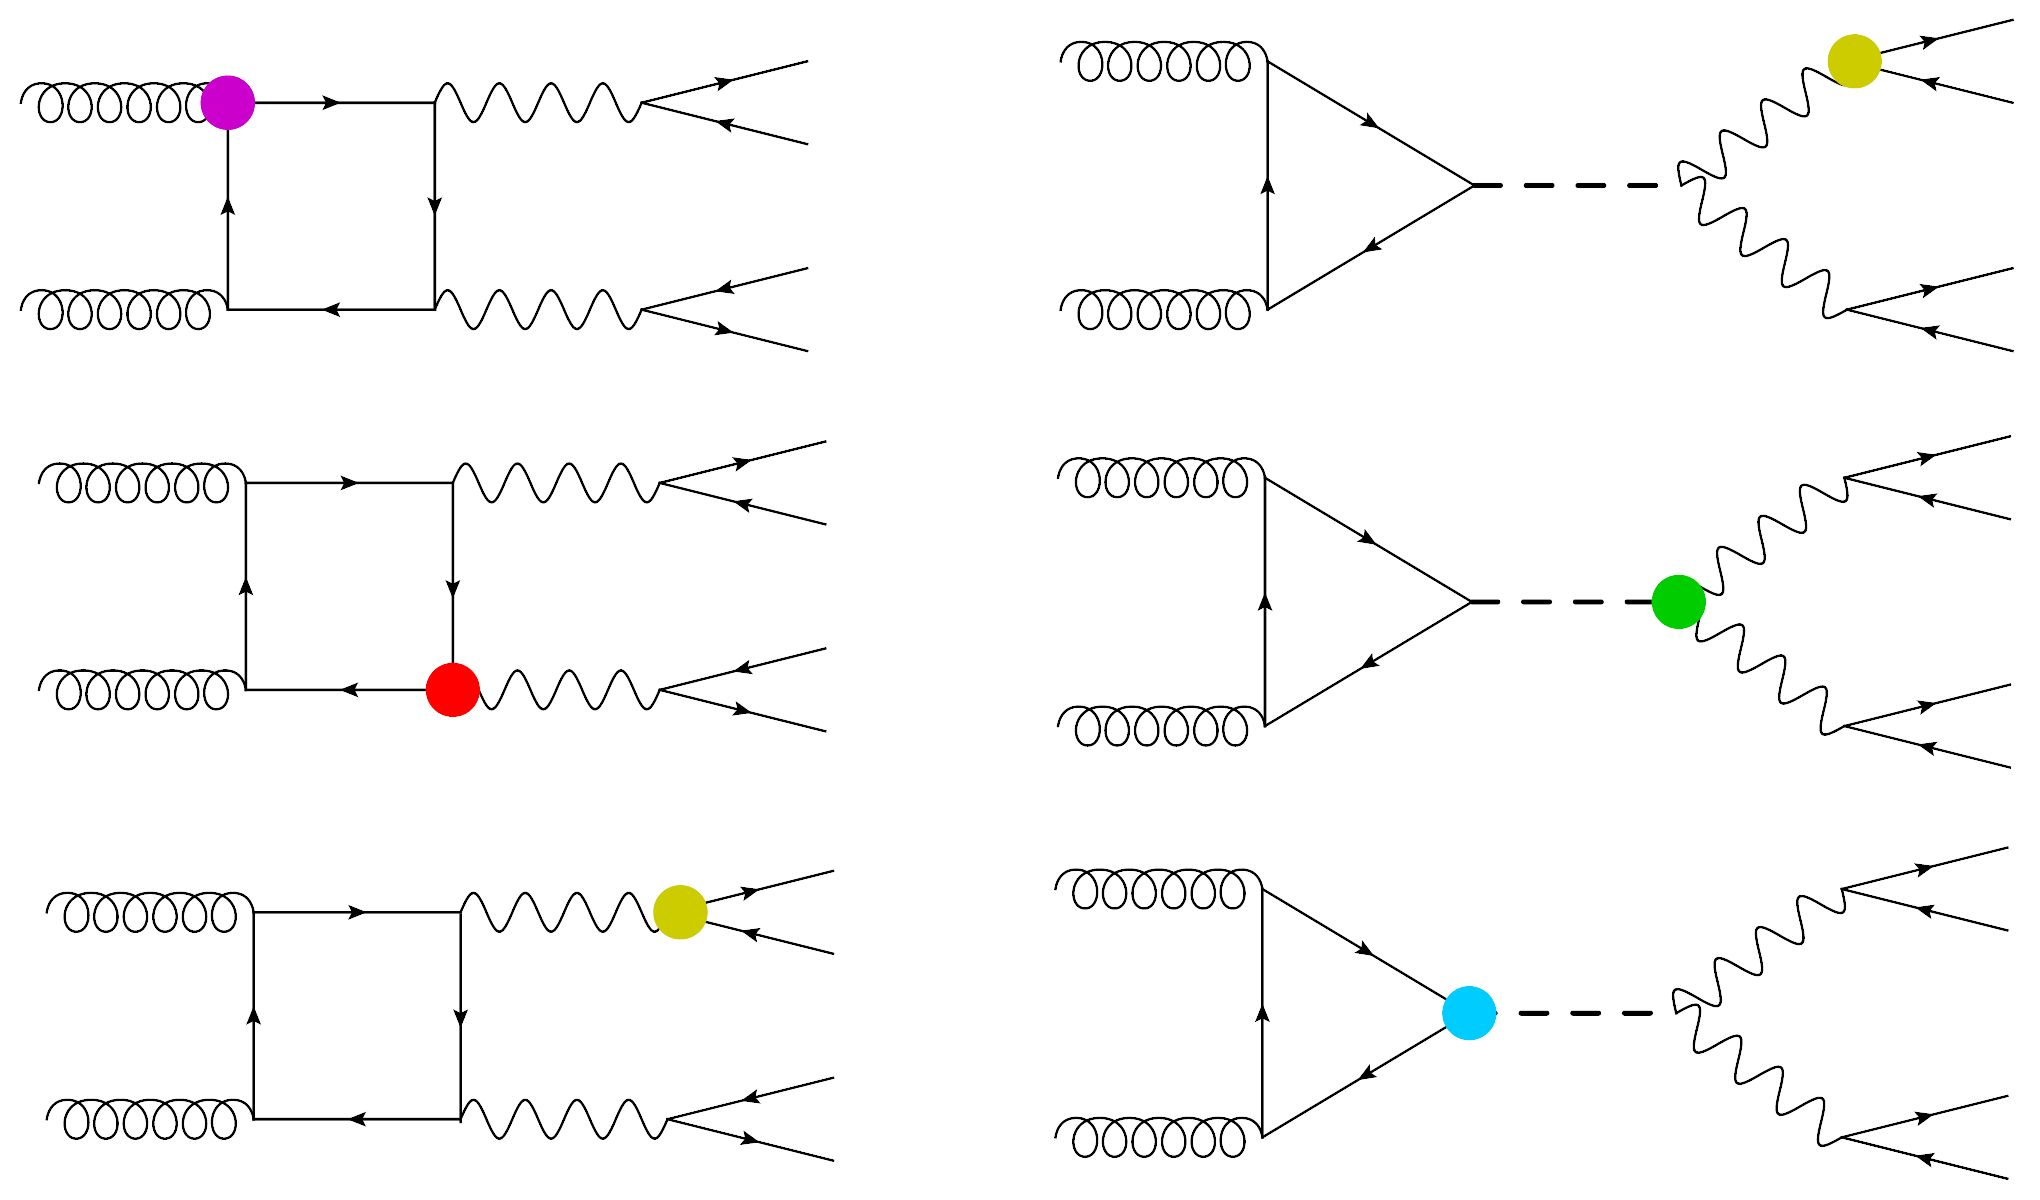
\includegraphics[width=0.9\textwidth,clip] {figures/EFTdiagrams.jpg}
\caption{Example Feynman diagrams for gluon fusion off-shell Higgs boson production (right) and corresponding background (left) with EFT insertions~\cite{offshellWGnote}.}
\label{fig:EFTdiagrams}
\end{figure}

% Anomalous contributions to the $HVV$ couplings may affect both the VBF and VH production mechanisms, as well as the Higgs boson decay into vector bosons. In the following discussion, we assume that the Higgs boson couples to two gauge bosons $VV$, such as $WW, ZZ, Z\gamma$, or $\gamma\gamma$, which in turn couple to fermions. These fermions appear either as four-lepton final states in Higgs boson decay, or as quarks and leptons in its production and in the decays of associated electroweak bosons.

% We assume that the Higgs boson does not couple to fermions via a new heavy state, which would generate a so-called contact interaction~\cite{Gonzalez-Alonso:2014eva,Greljo:2015sla}. However, the inclusion of amplitude terms corresponding to contact interactions is equivalent to testing anomalous $HVV$ couplings, as previously studied in~\cite{Khachatryan:2014kca}, under the assumption of flavor universality in $Vf\bar{f}$ interactions. Both approaches probe three general Lorentz-invariant tensor structures, with associated form factors $F_i(q_1^2,q_2^2)$, where $q_1$ and $q_2$ are the four-momenta of the two fermionic states, such as $(e^+e^-)$ and $(\mu^+\mu^-)$ in the $H \to e^+e^-\mu^+\mu^-$ decay, and analogous states in production.

% For this study, we fix all lepton and quark couplings to vector bosons to their SM values. While relaxing this assumption would allow for flavor non-universal couplings in the contact interaction terms, it would also introduce an excessive number of unconstrained parameters, making a meaningful test infeasible with the current data sample. We therefore restrict our analysis to the lowest-order operators, corresponding to the leading terms in the $(q_j^2/\Lambda^2)$ form-factor expansion, where $\Lambda$ denotes the energy scale of new physics.


% Even though we do not consider anomalous contributions in the \Hboson couplings to the SM particle
% in this version of analysis, let us still discuss those anomalous couplings for completeness, since they 
% will be constrained in the followup EFT analysis. 
% The treatment of anomalous couplings is based on a phenomenological framework 
% that describes the anomalous couplings of a Higgs-like boson
% to two gauge bosons, such as $\WW, \ZZ, \PZ\gamma, \gamma\gamma$ and $\glufu$.
% These couplings appear in either the production of the \Hboson or its decay,
% regardless of the \mell region in which the \Hboson is produced.
% The relationship in \Eq{eq:resonant} is therefore meant to imply concurrent variations
% in $\vv\PH$ couplings in both \onshell and \offshell regions.
% The coupling of the \Hboson to two gluons is assumed
% to be as in the SM, via quark loops with Yukawa couplings to quarks, where the contribution from the top-quark is dominant.
% This assumption is valid as long as the production is dominated
% by the top-quark loop and no new particles contribute to this loop.
% The Yukawa couplings also appear in direct interactions with fermion-antifermion pairs,
% such as in \ttH and \bbH productions. These interactions are of less importance in this study,
% since they are highly suppressed at high \offshell mass, but they are included in the analysis
% of the \onshell \Hboson production with similar assumptions as in the case of production via gluon fusion.
% Variation of the \HVV couplings, in either the \VBF or \VH~productions, or the \Hell decay,
% are allowed to depend on anomalous coupling contributions.

% In the following, we assume that the \Hboson couples to two gauge bosons \VV, such as
% \WW, \ZZ, $\PZ\gamma$ or $\gamma\gamma$, which in turn couple to fermions,
% either four leptons in \Hboson decay, or quarks or leptons in its production or in the decay
% of associated EW bosons. It is assumed that the \Hboson does not couple to fermions through
% a new heavy state, generating a so-called contact interaction~\cite{Gonzalez-Alonso:2014eva,Greljo:2015sla}.
% However, the inclusion of amplitude terms pertaining to contact interactions is equivalent to the
% anomalous \HVV couplings already tested~\cite{Khachatryan:2014kca} under the assumption
% of flavor universality in $\V\ffbar$ couplings.
% Both approaches test three general tensor structures allowed by Lorentz symmetry,
% with form factors $F_i(q_1^2,q_2^2)$ in front of each term,
% where $q_1$ and $q_2$ are the four-momenta of the two difermion states, such as $(\EE)$ and $(\MM)$ in the
% $\PH \to \EE\MM$ decay, and equivalent states in production. We also fix all lepton and quark couplings to vector bosons
% according to SM expectations. Relaxing this requirement would make it equivalent to flavor nonuniversal couplings of the contact terms,
% but would also introduce too many unconstrained parameters, which cannot be tested with the present data sample.
% Only the lowest order operators, or lowest order terms in the $(q_j^2/\Lambda^2)$ form-factor expansion, are tested,
% where $\Lambda$ is the energy scale of new physics.

\subsection{Amplitude EFT Couplings} \label{sec:amplitudeEFT}

We assume that the Higgs boson couples to two gauge bosons VV, such as WW, ZZ, Z$\gamma$, or $\gamma\gamma$, which in turn couple to fermions. These fermions appear either as four-lepton final states in the Higgs boson decay, or as quarks and leptons in its production and in the decays of associated electroweak bosons.

A general form of the signal scattering amplitude of the H boson with two vector bosons can be written in terms of polarization vectors $\epsilon_i$ and momenta $q_i$ of bosons $V_i$, with scalar tensor $f^{(i){\mu \nu}} = \epsilon_{i}^{\mu}q_{i}^{\nu} - \epsilon_{i}^\nu q_{i}^{\mu}$, as:

\begin{equation}
\label{eq:formfact-fullampl-spin0}
\begin{gathered}
A(HVV)\propto
\left[ a_{1}^{VV}
+ \frac{\kappa_1^{VV}q_{1}^2 + \kappa_2^{VV} q_{2}^{2}}{\left(\Lambda_{1}^{VV} \right)^{2}}
+ \frac{\kappa_3^{VV}(q_{1} + q_{2})^{2}}{\left(\Lambda_{Q}^{VV} \right)^{2}}
\right]
m_{V1}^2 \epsilon_{V1}^* \epsilon_{V2}^* \\
+ a_{2}^{VV}  f_{\mu \nu}^{*(1)}f^{*(2),\mu\nu}
+ a_{3}^{VV}   f^{*(1)}_{\mu \nu} {\tilde f}^{*(2),\mu\nu},
\end{gathered}
\end{equation}

such that the scales of BSM physics are set by $\Lambda_{1}$ and $\Lambda_{Q}$, and the $a_{2}^{VV}$ and $a_{3}^{VV}$ scaled terms provide CP-even and CP-odd contributions, which may be sensitive to evidence of CP violation. Figure \ref{fig:EFTdiagrams2} highlights the double $HVV$ vertex present in our electroweak Feynman diagrams.

\begin{figure}[!hbt]
\centering
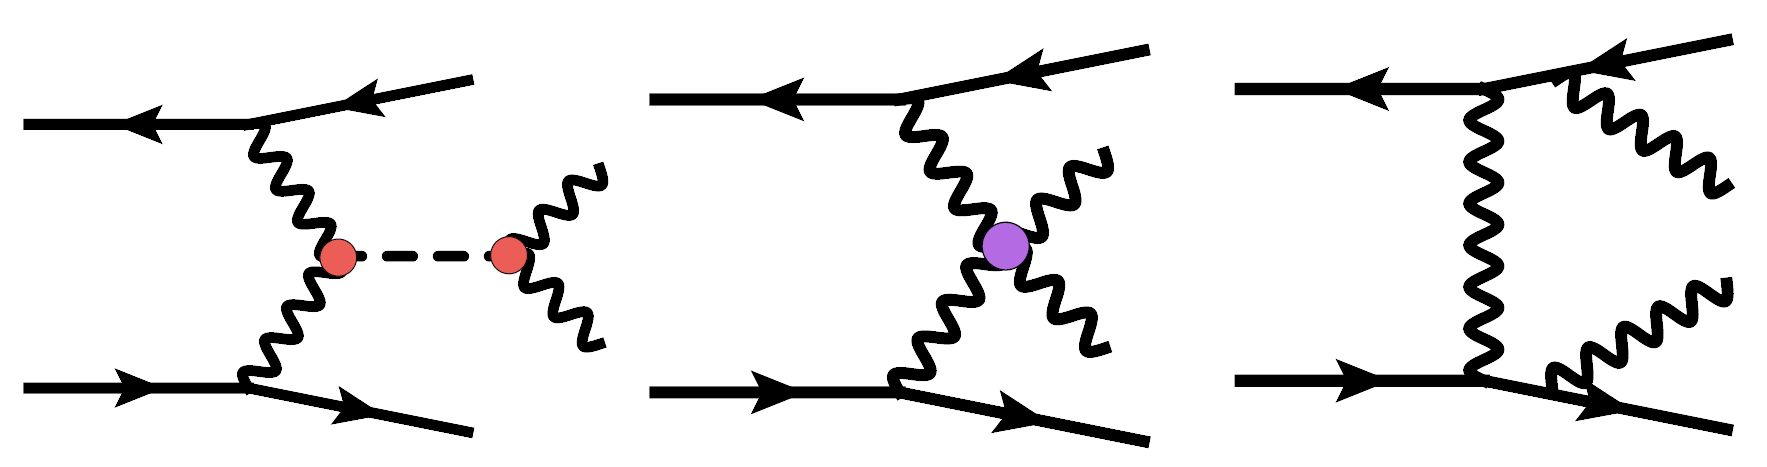
\includegraphics[width=0.8\textwidth,clip] {figures/EFTdiagrams2.jpg}
\caption{Example Feynman diagrams for electroweak off-shell Higgs boson production (left), vector boson scattering (VBS) (center), and additional background (right) with EFT insertions~\cite{offshellWGnote}.}
\label{fig:EFTdiagrams2}
\end{figure}

When at least one of the gauge bosons $V$ is massive, $m_{V1}$ is the pole mass of that gauge boson. All the $a_i^{VV}$ (which denotes $a_{1}^{VV}$, $1/\Lambda_{1}$, $1/\Lambda_{Q}$, $a_{2}^{VV}$, and $a_{3}^{VV}$) terms act as coupling-strength modifiers on their corresponding contributions to the amplitude. 

% Under the assumption that the couplings are constant and real, Equation \ref{eq:formfact-fullampl-spin0} is equivalent
% to an effective Lagrangian notation. Therefore, in this paper, the real coupling constants are tested.
% The above approach allows a sufficiently general test of the \(H \to 4\ell\)
% kinematics in decay and equivalent kinematics in production, as discussed below, including production
% and decay of virtual intermediate photons. If deviations from the SM are detected,
% a more detailed study of $F_i(q_1^2,q_2^2)$ could be performed, eventually providing a measurement of the
% double-differential cross section for each tensor structure tested.

Instead of constraining any $a_i$ directly, we can constrain the fractional contribution of its corresponding term to the signal scattering amplitude of the Higgs boson, as a ratio of observable cross sections $f_{ai}$. In Equation~\ref{eq:formfact-fullampl-spin0}, pure SM behavior is described by $a_{1}^{VV}$ alone. This would correspond to a measurement of $f_{a_1}=1$. If, for example, we took $f_{a_1}=0.5$, then we would have a $50\%$ contribution to our overall cross section from the SM and $50\%$ from BSM physics.

This parameterization via $f_{ai}$ has the benefit of being invariant to the $a_n$ coupling scale, and having values bounded by 0 and 1. Also, in experimental measurements of $f_{ai}$ most systematic uncertainties cancel in the ratios to give us a cleaner measurement~\cite{2020}. We define ratio $f_{ai}$ and phase $\phi_{ai}$ as:

\begin{equation}
\label{eq:faiandphase}
\begin{gathered}
f_{ai} = \frac{|a_i|^2 \sigma_i}{\sum_{j=1,2,3...}|a_i|^2 \sigma_j},   \phi_{ai} = arg(\frac{a_i}{a_1}).
\end{gathered}
\end{equation}

\subsection{Kappa Framework Couplings} \label{sec:kappa}

Another representation of the Higgs boson couplings utilizes the so-called $\kappa$ framework, in which couplings of 
the Higgs boson to the SM particles are modified by a scale factor $\kappa_i$ for each particle $i$.

As previously discussed, SM-like behavior implies the top quark's predominance in the gluon fusion loop during Higgs boson production. If there are additional contributions in this loop, such as from undiscovered heavy particles, the probability distribution for Higgs boson production in the off-shell region would change. To model this, one could introduce a heavy quark~$\mathrm{Q}$ with coupling strength to the \Hboson $\kappa_\mathrm{Q}$~\cite{Gritsan:2020pib,Davis:2021tiv}.

In the framework of effective field theories, the contribution from $\mathrm{Q}$ can be reasonably interpreted as a point-like interaction which integrates all effects from heavy particles present in the loop.
One can include both top and bottom quarks in the loop, characterized by the coupling strength $\kappa_\mathrm{q}$, 
where $\kappa_\mathrm{q}=1$ corresponds to the SM. Similarly, $\kappa_\mathrm{V}$ is the \Hboson coupling strength to the Z and W bosons, which impact EW production and \Hboson decay and where $\kappa_\mathrm{V}=1$ in the SM. 

As described in Equation~\ref{eq:resonant}, we usually parameterize our model in terms of signal strength. In this analysis, we use $\mu_F$ for Higgs boson production mechanisms driven by fermion couplings, i.e. production via ggH or in association with a t$\bar{\text{t}}$ (t$\bar{\text{t}}$H) or b$\bar{\text{b}}$ pair (b$\bar{\text{b}}$H). 
For EW production, i.e., production via vector boson fusion (VBF) or in association with a W or Z boson (VH), the signal strength is denoted as $\mu_V$.

The $\kappa$ framework requires a re-parameterization in terms of $\kappa_\mathrm{q}$, $\kappa_\mathrm{Q}$, and $\kappa_\mathrm{V}$~\cite{Davis:2021tiv}:
\begin{equation}
\begin{aligned}
& \mu_V=\kappa_V^4\times\frac{\Gamma_0}{\Gamma} \\
& \mu_F=\kappa_q^2\kappa_V^2\times\frac{\Gamma_0}{\Gamma}
\end{aligned}
\label{eq:KappaMu}
\end{equation}
where $\Gamma_0$ is the reference value of the Higgs boson width used in
simulation, and
\begin{equation}
\begin{aligned}
& \kappa_Z = \kappa_W = \kappa_V= \mathrm{sign}(\mu_V)\left(|\mu_V|\frac{\Gamma}{\Gamma_0}\right)^\frac{1}{4} \\
& \kappa_t = \kappa_b = \kappa_q= \mathrm{sign}(\mu_F)|\mu_F|^\frac{1}{2} \left(\frac{1}{|\mu_V|}\frac{\Gamma}{\Gamma_0}\right)^\frac{1}{4}
\end{aligned}
\label{eq:KappaMu2}
\end{equation}
The bulk of this thesis focuses on measurements of the SM Higgs boson, but it will also include an extension of the analysis which sets constraints on these $\kappa$ framework coupling strengths. It should become apparent that this analysis also sets the stage for upcoming measurements of anomalous coupling strengths in our amplitude basis, presented in Section~\ref{sec:amplitudeEFT}.

% On-shell pdf:
% \begin{equation}
% \begin{aligned}
% \mathcal{P}_{k}(\vec{x};\vec{\xi}_{k},\vec\zeta) =& \frac{(0.22 \kappa_Z^2 + 0.78\kappa_W^2 )\kappa_Z^2 \Gamma_0}{\Gamma_H}\mathcal{P}_{k}^\text{VBF sig} ( \vec{x};\vec{\xi}_{k}) \\
% &+\frac{( 0.3916\kappa_Z^2 + 0.6084\kappa_W^2 )\kappa_Z^2\Gamma_0}{\Gamma_H}\mathcal{P}_{k}^\text{VH sig} ( \vec{x};\vec{\xi}_{k}) \\
% &+\frac{\kappa_g^2\kappa_Z^2\Gamma_0}{\Gamma_H} \mathcal{P}_{k}^\text{ggf sig} ( \vec{x};\vec{\xi}_{k}) \\
% &+\frac{\kappa_t^2\kappa_Z^2\Gamma_0}{\Gamma_H} \mathcal{P}_{k}^\text{ttH sig} ( \vec{x};\vec{\xi}_{k}) \\
% &+ \mathcal{P}_{k}^\text{bkg}( \vec{x};\vec{\xi}_{k}),
% \end{aligned}
% \label{eq:Kappaponshell}
% \end{equation}

% Equation taken from~\cite{PhysRevD.105.096027}:
% \begin{equation}
% \begin{aligned}
% \kappa_g^2 =& 1.1068\kappa_t^2 + 0.0082\kappa_b^2 -0.1150\kappa_t\kappa_b \\
%             &+1.0298\kappa_Q^2 + 2.1357\kappa_t\kappa_Q - 0.1109\kappa_b\kappa_Q
% \end{aligned}
% \label{eq:kg2}
% \end{equation}

% Off-shell pdf:
% \begin{equation}
% \begin{aligned}
% \mathcal{P}_{k}(\vec{x};\vec{\xi}_{k},\vec\zeta) =&\kappa_Z^4~\mathcal{P}_{k}^{(VBF+VH)_{Z} \text{sig}} ( \vec{x};\vec{\xi}_{k}) \\
% &+\kappa_W^2\kappa_Z^2~\mathcal{P}_{k}^{(VBF+VH)_W \text{sig}} ( \vec{x};\vec{\xi}_{k})\\
% &+\kappa_W\kappa_Z^3~\mathcal{P}_{k}^{(VBF+VH)_{WZ} \text{sig}} ( \vec{x};\vec{\xi}_{k})  \\
% &+\kappa_Z^2~\mathcal{P}_{k}^{(VBF+VH)_Z \text{int}} ( \vec{x};\vec{\xi}_{k})  \\
% &+\kappa_W\kappa_Z~\mathcal{P}_{k}^{(VBF+VH)_W \text{int}} ( \vec{x};\vec{\xi}_{k})  \\
% &+\kappa_t^2\kappa_Z^2~\mathcal{P}_{k}^{ggF_{t} \text{sig}} ( \vec{x};\vec{\xi}_{k}) \\
% &+\kappa_Q^2\kappa_Z^2~\mathcal{P}_{k}^{ggF_{Q} \text{sig}} ( \vec{x};\vec{\xi}_{k}) \\
% &+\kappa_t\kappa_Q\kappa_Z^2~\mathcal{P}_{k}^{ggF_{tQ} \text{sig}} ( \vec{x};\vec{\xi}_{k}) \\
% &+(\kappa_t\kappa_Z)~\mathcal{P}_{k}^{ggF_{top} \text{int}} ( \vec{x};\vec{\xi}_{k}) \\
% &+(\kappa_Q\kappa_Z)~\mathcal{P}_{k}^{ggF_{Q} \text{int}} ( \vec{x};\vec{\xi}_{k}) \\
% &+\frac{\kappa_Z^4\Gamma_0}{\Gamma_H}~\mathcal{P}_{k}^\text{cross} ( \vec{x};\vec{\xi}_{k}) \\
% &+ \mathcal{P}_{k}^\text{bkg} ( \vec{x};\vec{\xi}_{k}),
% \end{aligned}
% \label{eq:Kappapoffshell}
% \end{equation}